% ============================================================================
% I2C Communication with BMP280 — Bare-Metal on STM32F446RE
% A Comprehensive, Colorful Guide for Lab Exam Preparation
% ============================================================================

\documentclass[12pt, a4paper]{article}

% ── Encoding & Fonts ────────────────────────────────────────────────────────
\usepackage[utf8]{inputenc}
\usepackage[T1]{fontenc}
\usepackage{lmodern}

% ── Page Geometry ───────────────────────────────────────────────────────────
\usepackage[margin=2cm, top=2.5cm, bottom=2.5cm, headheight=25pt]{geometry}

% ── Colors ──────────────────────────────────────────────────────────────────
\usepackage[dvipsnames, svgnames, x11names]{xcolor}

% Custom palette
\definecolor{deepblue}{HTML}{1A237E}
\definecolor{accentblue}{HTML}{1565C0}
\definecolor{lightbluebg}{HTML}{E3F2FD}
\definecolor{warnorange}{HTML}{E65100}
\definecolor{successgreen}{HTML}{1B5E20}
\definecolor{hintpurple}{HTML}{6A1B9A}
\definecolor{codebg}{HTML}{F5F5F5}
\definecolor{codeframe}{HTML}{BDBDBD}
\definecolor{sectioncolor}{HTML}{0D47A1}
\definecolor{subsectioncolor}{HTML}{1565C0}
\definecolor{registerbg}{HTML}{FFF3E0}
\definecolor{tipbg}{HTML}{E8F5E9}
\definecolor{warnbg}{HTML}{FBE9E7}
\definecolor{altbg}{HTML}{F3E5F5}
\definecolor{darkcodebg}{HTML}{263238}

% ── Packages ────────────────────────────────────────────────────────────────
\usepackage{listings}
\usepackage{tcolorbox}
\tcbuselibrary{listings, skins, breakable}
\usepackage{tikz}
\usetikzlibrary{arrows.meta, positioning, shapes.geometric, calc, decorations.pathmorphing, decorations.pathreplacing, backgrounds, fit}
\usepackage{booktabs}
\usepackage{tabularx}
\usepackage{multirow}
\usepackage{enumitem}
\usepackage{hyperref}
\usepackage{fancyhdr}
\usepackage{titlesec}
\usepackage{amsmath}
\usepackage{fontawesome5}
\usepackage{pifont}
\usepackage{float}
\usepackage{graphicx}
\usepackage{array}
\usepackage{colortbl}

% ── Hyperlinks ──────────────────────────────────────────────────────────────
\hypersetup{
    colorlinks=true,
    linkcolor=accentblue,
    urlcolor=hintpurple,
    citecolor=successgreen,
    pdfauthor={CSE-2206 Microcontroller Lab},
    pdftitle={I2C Communication with BMP280 - Bare-Metal Guide},
}

% ── Section Formatting ─────────────────────────────────────────────────────
\titleformat{\section}
    {\LARGE\bfseries\color{sectioncolor}}
    {\thesection.}{0.5em}{}
    [\vspace{-0.5em}\textcolor{sectioncolor}{\rule{\linewidth}{1.5pt}}]

\titleformat{\subsection}
    {\Large\bfseries\color{subsectioncolor}}
    {\thesubsection}{0.5em}{}

\titleformat{\subsubsection}
    {\large\bfseries\color{hintpurple}}
    {\thesubsubsection}{0.5em}{}

% ── Header/Footer ──────────────────────────────────────────────────────────
\pagestyle{fancy}
\fancyhf{}
\fancyhead[L]{\textcolor{accentblue}{\textbf{CSE-2206} $\mid$ I2C Bare-Metal Guide}}
\fancyhead[R]{\textcolor{accentblue}{BMP280 Sensor}}
\fancyfoot[C]{\textcolor{gray}{--- Page \thepage\ ---}}
\renewcommand{\headrulewidth}{1pt}
\renewcommand{\headrule}{\hbox to\headwidth{\textcolor{accentblue}{\leaders\hrule height \headrulewidth\hfill}}}

% ── Code Listing Style ─────────────────────────────────────────────────────
\lstdefinestyle{CStyle}{
    language=C,
    basicstyle=\small\ttfamily,
    keywordstyle=\bfseries\color{deepblue},
    stringstyle=\color{OrangeRed},
    commentstyle=\itshape\color{ForestGreen},
    identifierstyle=\color{black},
    numberstyle=\tiny\color{gray},
    numbers=left,
    numbersep=8pt,
    breaklines=true,
    showstringspaces=false,
    tabsize=4,
    frame=none,
    xleftmargin=1em,
    morekeywords={uint8_t, uint16_t, uint32_t, int8_t, int16_t, int32_t, int64_t, void},
    literate={->}{{{\color{RedOrange}->}}}2
             {<<}{{{\color{RedOrange}<<}}}2
             {>>}{{{\color{RedOrange}>>}}}2
             {|=}{{{\color{RedOrange}|=}}}2
             {&=}{{{\color{RedOrange}\&=}}}2,
}

% ── tcolorbox Styles ───────────────────────────────────────────────────────
\newtcolorbox{codebox}[1][]{
    enhanced, breakable,
    colback=codebg, colframe=codeframe,
    arc=4pt, boxrule=0.8pt,
    fonttitle=\bfseries\color{white},
    coltitle=white, colbacktitle=accentblue,
    title={#1},
    left=2pt, right=2pt, top=2pt, bottom=2pt,
}

\newtcolorbox{conceptbox}[1][]{
    enhanced, breakable,
    colback=lightbluebg, colframe=accentblue,
    arc=6pt, boxrule=1.2pt,
    fonttitle=\bfseries\large\color{white},
    coltitle=white, colbacktitle=accentblue,
    title={\faIcon{lightbulb}\ \ #1},
    left=8pt, right=8pt, top=4pt, bottom=4pt,
    shadow={2pt}{-2pt}{0pt}{black!20},
}

\newtcolorbox{tipbox}[1][]{
    enhanced, breakable,
    colback=tipbg, colframe=successgreen,
    arc=4pt, boxrule=1pt,
    fonttitle=\bfseries\color{white},
    coltitle=white, colbacktitle=successgreen,
    title={\faIcon{check-circle}\ \ #1},
    left=8pt, right=8pt, top=4pt, bottom=4pt,
}

\newtcolorbox{warnbox}[1][]{
    enhanced, breakable,
    colback=warnbg, colframe=warnorange,
    arc=4pt, boxrule=1pt,
    fonttitle=\bfseries\color{white},
    coltitle=white, colbacktitle=warnorange,
    title={\faIcon{exclamation-triangle}\ \ #1},
    left=8pt, right=8pt, top=4pt, bottom=4pt,
}

\newtcolorbox{altbox}[1][]{
    enhanced, breakable,
    colback=altbg, colframe=hintpurple,
    arc=4pt, boxrule=1pt,
    fonttitle=\bfseries\color{white},
    coltitle=white, colbacktitle=hintpurple,
    title={\faIcon{exchange-alt}\ \ #1},
    left=8pt, right=8pt, top=4pt, bottom=4pt,
}

\newtcolorbox{registerbox}[1][]{
    enhanced, breakable,
    colback=registerbg, colframe=warnorange,
    arc=4pt, boxrule=1pt,
    fonttitle=\bfseries\color{white},
    coltitle=white, colbacktitle=warnorange,
    title={\faIcon{microchip}\ \ #1},
    left=8pt, right=8pt, top=4pt, bottom=4pt,
}

% ── Document ────────────────────────────────────────────────────────────────
\begin{document}

% ╔══════════════════════════════════════════════════════════════════════════╗
% ║                           TITLE PAGE                                    ║
% ╚══════════════════════════════════════════════════════════════════════════╝
\begin{titlepage}

\begin{tikzpicture}[remember picture, overlay]
    % Background gradient rectangles
    \fill[deepblue] (current page.south west) rectangle (current page.north east);
    \fill[accentblue, opacity=0.7] ([yshift=-3cm]current page.north west) rectangle ([yshift=-12cm]current page.north east);
    \fill[white, opacity=0.05] ([yshift=-5cm]current page.north west) -- ([yshift=-7cm]current page.north east) -- ([yshift=-12cm]current page.north east) -- ([yshift=-10cm]current page.north west) -- cycle;
    
    % Decorative circles
    \foreach \r/\o in {4/0.03, 6/0.02, 8/0.015} {
        \fill[white, opacity=\o] ([xshift=3cm, yshift=-8cm]current page.north east) circle (\r cm);
    }
    \foreach \r/\o in {3/0.04, 5/0.025, 7/0.015} {
        \fill[white, opacity=\o] ([xshift=-2cm, yshift=5cm]current page.south west) circle (\r cm);
    }
    
    % Title text
    \node[anchor=center, text=white] at ([yshift=-5cm]current page.north) {
        \begin{minipage}{0.85\textwidth}
            \centering
            {\fontsize{14}{16}\selectfont\textsc{CSE-2206: Microcontroller Lab}}\\[0.8cm]
            {\fontsize{36}{40}\selectfont\textbf{I2C Communication}}\\[0.3cm]
            {\fontsize{36}{40}\selectfont\textbf{with BMP280}}\\[0.6cm]
            {\fontsize{16}{20}\selectfont\textcolor{cyan!60!white}{Bare-Metal Implementation on STM32F446RE}}\\[0.3cm]
            {\fontsize{12}{14}\selectfont\textcolor{white!70}{A Comprehensive Function-by-Function Guide}}
        \end{minipage}
    };
    
    % Separator line
    \draw[white, line width=1.5pt] ([xshift=3cm, yshift=-10.5cm]current page.north west) -- ([xshift=-3cm, yshift=-10.5cm]current page.north east);
    
    % Info box
    \node[anchor=center, text=white] at ([yshift=-14cm]current page.north) {
        \begin{minipage}{0.7\textwidth}
            \centering
            {\large\textbf{Assignment 03 --- LAB 02(A)}}\\[0.6cm]
            \begin{tabular}{rl}
                \textcolor{cyan!60!white}{\faIcon{microchip}} & \textbf{MCU:} STM32F446RE (Nucleo-64) \\[0.3cm]
                \textcolor{cyan!60!white}{\faIcon{plug}} & \textbf{Sensor:} BMP280 (Bosch) \\[0.3cm]
                \textcolor{cyan!60!white}{\faIcon{exchange-alt}} & \textbf{Protocol:} I2C (Standard Mode, 100\,kHz) \\[0.3cm]
                \textcolor{cyan!60!white}{\faIcon{code}} & \textbf{Approach:} Bare-Metal (No HAL / No Library) \\
            \end{tabular}
        \end{minipage}
    };
    
    % Bottom decoration
    \fill[white, opacity=0.1] (current page.south west) rectangle ([yshift=2cm]current page.south east);
    \node[anchor=south, text=white!60, font=\small] at ([yshift=0.5cm]current page.south) {Lab Exam Preparation Guide};
\end{tikzpicture}
\end{titlepage}

% ── Table of Contents ───────────────────────────────────────────────────────
\newpage
\tableofcontents
\newpage

% ╔══════════════════════════════════════════════════════════════════════════╗
% ║                SECTION 1: WHAT IS I2C?                                  ║
% ╚══════════════════════════════════════════════════════════════════════════╝
\section{What Is I2C? --- The Big Picture}

\begin{conceptbox}[Understanding I2C in Simple Terms]
\textbf{I2C (Inter-Integrated Circuit)} is a \textbf{two-wire} communication protocol that lets a \textbf{master} device (our STM32 microcontroller) talk to one or more \textbf{slave} devices (our BMP280 sensor) using just two lines:

\begin{itemize}[leftmargin=2em]
    \item \textbf{\textcolor{accentblue}{SCL (Serial Clock Line)}} --- The master generates a clock signal here. Every ``tick'' of this clock means one bit of data is being transferred.
    \item \textbf{\textcolor{successgreen}{SDA (Serial Data Line)}} --- Actual data flows here, in both directions (master $\leftrightarrow$ slave).
\end{itemize}

Think of it like a \textbf{telephone call}: the master dials a number (slave address), waits for the other party to pick up (ACK), then either speaks (writes data) or listens (reads data).
\end{conceptbox}

\subsection{How I2C Works --- Step by Step}

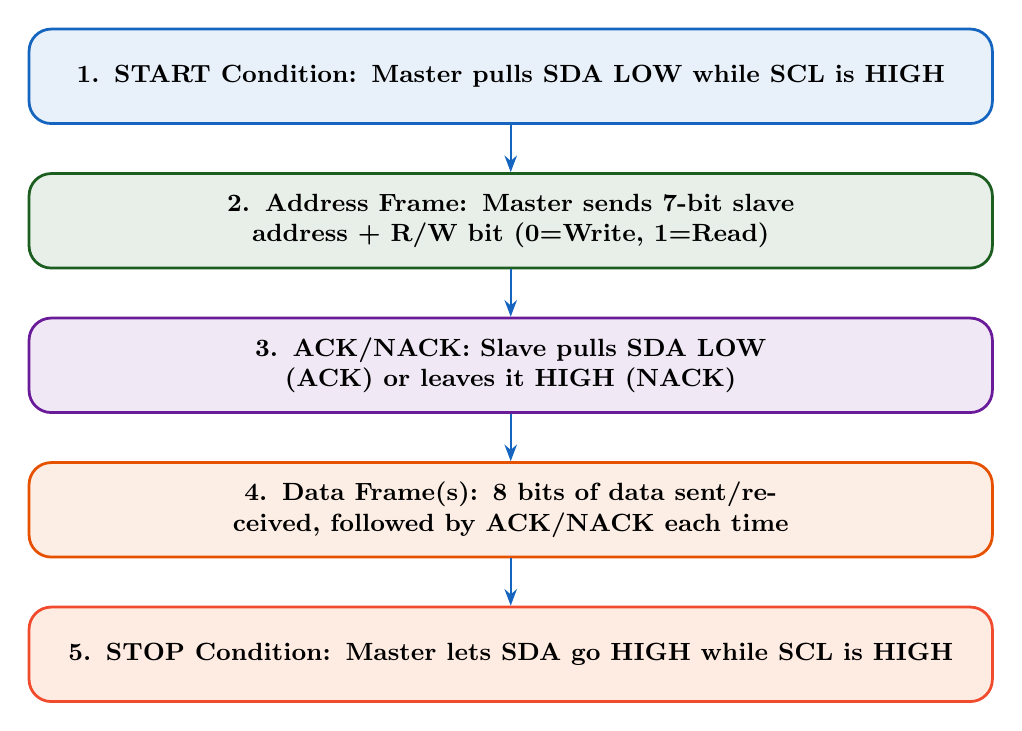
\begin{tikzpicture}[
    node distance=0.6cm and 2cm,
    step/.style={rectangle, rounded corners=8pt, draw=#1, fill=#1!10, text width=12cm, minimum height=1.2cm, align=center, font=\small\bfseries, line width=1pt},
    arrow/.style={-{Stealth[length=6pt]}, thick, color=accentblue},
]
    \node[step=accentblue] (s1) {1. \textbf{START Condition}: Master pulls SDA LOW while SCL is HIGH};
    \node[step=successgreen, below=of s1] (s2) {2. \textbf{Address Frame}: Master sends 7-bit slave address + R/W bit (0=Write, 1=Read)};
    \node[step=hintpurple, below=of s2] (s3) {3. \textbf{ACK/NACK}: Slave pulls SDA LOW (ACK) or leaves it HIGH (NACK)};
    \node[step=warnorange, below=of s3] (s4) {4. \textbf{Data Frame(s)}: 8 bits of data sent/received, followed by ACK/NACK each time};
    \node[step=RedOrange, below=of s4] (s5) {5. \textbf{STOP Condition}: Master lets SDA go HIGH while SCL is HIGH};
    
    \draw[arrow] (s1) -- (s2);
    \draw[arrow] (s2) -- (s3);
    \draw[arrow] (s3) -- (s4);
    \draw[arrow] (s4) -- (s5);
\end{tikzpicture}

\subsection{Why I2C? (Compared to Other Protocols)}

\begin{center}
\renewcommand{\arraystretch}{1.3}
\begin{tabularx}{\textwidth}{>{\centering\arraybackslash\bfseries\columncolor{accentblue!15}}p{2.5cm} >{\centering\arraybackslash}X >{\centering\arraybackslash}X >{\centering\arraybackslash}X}
\toprule
\rowcolor{accentblue!30}
\textbf{Feature} & \textbf{I2C} & \textbf{SPI} & \textbf{UART} \\
\midrule
Wires Needed & \textcolor{successgreen}{\textbf{2}} (SDA, SCL) & 4+ (MOSI, MISO, SCK, CS) & 2 (TX, RX) \\
\rowcolor{gray!5}
Multi-Slave? & \textcolor{successgreen}{\textbf{Yes}} (via address) & Yes (extra CS per slave) & No (point-to-point) \\
Speed & Up to 3.4\,Mbps & Up to 50+ Mbps & Up to 5\,Mbps \\
\rowcolor{gray!5}
Complexity & Medium & Low & Low \\
Acknowledgment & \textcolor{successgreen}{\textbf{Built-in}} (ACK/NACK) & None & None \\
\bottomrule
\end{tabularx}
\end{center}

\begin{tipbox}[Why BMP280 uses I2C]
The BMP280 sensor only needs to send a few bytes of data (temperature, pressure). I2C's low wire count (just 2 wires!) makes wiring simple, and its built-in addressing lets you connect multiple sensors on the same bus.
\end{tipbox}

% ╔══════════════════════════════════════════════════════════════════════════╗
% ║                SECTION 2: HARDWARE WIRING                               ║
% ╚══════════════════════════════════════════════════════════════════════════╝
\section{Hardware Wiring \& Pin Configuration}

\begin{registerbox}[Physical Connections]
\renewcommand{\arraystretch}{1.4}
\begin{tabularx}{\textwidth}{>{\centering\bfseries\color{accentblue}}p{3cm} >{\centering}p{3.5cm} X}
\toprule
\rowcolor{warnorange!15}
\textbf{BMP280 Pin} & \textbf{Nucleo Pin} & \textbf{Purpose} \\
\midrule
VCC & 3V3 & Power supply (3.3V) \\
\rowcolor{gray!5}
GND & GND & Ground reference \\
SCL & PB8 / D15 & I2C clock line \\
\rowcolor{gray!5}
SDA & PB9 / D14 & I2C data line \\
CSB & Wired to VCC & Selects I2C mode (HIGH = I2C, LOW = SPI) \\
\rowcolor{gray!5}
SDO & Wired to GND & Sets I2C address to \texttt{0x76} (LOW = 0x76, HIGH = 0x77) \\
\bottomrule
\end{tabularx}
\end{registerbox}

\begin{warnbox}[Critical Wiring Note]
\begin{itemize}[leftmargin=1.5em]
    \item \textbf{CSB must be HIGH} (tied to VCC) to enable I2C mode. If CSB is LOW, the BMP280 switches to SPI mode.
    \item \textbf{SDO = GND} forces the slave address to \texttt{0x76}. If SDO = VCC, the address becomes \texttt{0x77}. This lets you connect \textbf{two} BMP280 sensors on the same I2C bus with different addresses!
    \item I2C lines need \textbf{open-drain outputs with pull-up resistors} so the bus stays HIGH when idle.
\end{itemize}
\end{warnbox}

% ╔══════════════════════════════════════════════════════════════════════════╗
% ║                SECTION 3: REGISTER MAP                                  ║
% ╚══════════════════════════════════════════════════════════════════════════╝
\section{BMP280 Register Map \& Macros}

Every sensor has internal \textbf{registers} --- small memory locations that you read from or write to in order to control the sensor or get data. Here are the registers used in our code:

\begin{center}
\renewcommand{\arraystretch}{1.35}
\begin{tabularx}{\textwidth}{>{\ttfamily\bfseries\color{deepblue}\centering\arraybackslash}p{2cm} >{\centering\arraybackslash}p{4.8cm} X}
\toprule
\rowcolor{accentblue!20}
\textbf{Address} & \textbf{Macro Name} & \textbf{What It Does} \\
\midrule
0xD0 & REGISTER\_CHIP\_ID & Returns chip ID: \texttt{0x58} for BMP280, \texttt{0x60} for BME280 \\
\rowcolor{gray!5}
0xE0 & REGISTER\_RESET & Write \texttt{0xB6} here to soft-reset the sensor \\
0xF2 & REGISTER\_CTRL\_HUM & Humidity oversampling control (BME280 only) \\
\rowcolor{gray!5}
0xF3 & REGISTER\_STATUS & Reports if a measurement is in progress \\
0xF4 & REGISTER\_CONTROL\_MEASURE & Temperature/Pressure oversampling + operating mode \\
\rowcolor{gray!5}
0xF5 & REGISTER\_CONFIGURE & IIR filter coefficient + standby time \\
0xF7 & REGISTER\_PRESSURE\_MSB & Start of raw pressure data (3 bytes: 0xF7--0xF9) \\
\rowcolor{gray!5}
0x88 & REGISTER\_CALIBRATION\_START & Start of calibration data block (24 bytes) \\
\bottomrule
\end{tabularx}
\end{center}

\begin{codebox}[\faIcon{code}\ \ Register Macros in Code]
\begin{lstlisting}[style=CStyle]
#define BME_P280_REGISTER_CHIP_ID           0xD0
#define BME_P280_REGISTER_RESET             0xE0
#define BME_P280_REGISTER_CONTROL_MEASURE   0xF4
#define BME_P280_REGISTER_CONFIGURE         0xF5
#define BME_P280_REGISTER_PRESSURE_MSB      0xF7
#define BME_P280_REGISTER_CALIBRATION_START  0x88
#define BME_P280_RESET_VALUE                0xB6

// Control Measure: Temp osrs x2, Press osrs x16, Normal mode
#define BME_P280_CONTROL_MEASURE_VALUE  ((2U << 5) | (5U << 2) | 3U)
// = 0b01_010_11 = 0x57

// Configure: IIR filter coeff x16, Standby 125ms
#define BME_P280_CONFIGURE_VALUE  ((4U << 5) | (4U << 2))
// = 0b100_100_00 = 0x90
\end{lstlisting}
\end{codebox}

\begin{conceptbox}[Understanding the Control Measure Register (0xF4)]
The \texttt{ctrl\_meas} register at \texttt{0xF4} is packed as:

\begin{center}
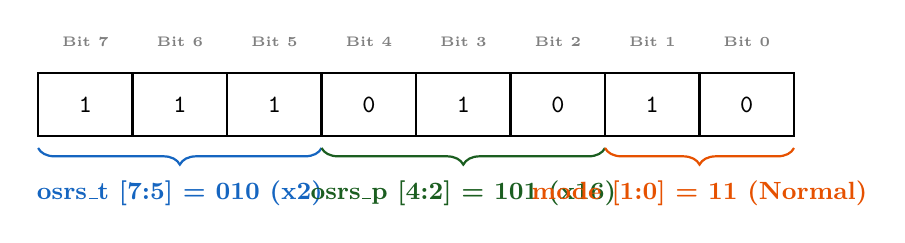
\begin{tikzpicture}
    \def\w{1.2}
    % Bit labels
    \foreach \b in {7,6,5,4,3,2,1,0} {
        \node[font=\tiny\bfseries, text=gray] at ({(7-\b)*\w + \w/2}, 1.2) {Bit \b};
    }
    % Boxes
    \foreach \b in {0,...,7} {
        \draw[thick, fill=white] (\b*\w, 0) rectangle +(\w, 0.8);
    }
    % Values for 0x57 = 0101 0111
    \foreach \b/\v in {0/0, 1/1, 2/0, 3/1, 4/0, 5/1, 6/1, 7/1} {
        \node[font=\small\ttfamily\bfseries] at ({(7-\b)*\w + \w/2}, 0.4) {\v};
    }
    % Group labels
    \draw[decorate, decoration={brace, amplitude=6pt, mirror}, thick, accentblue] (0, -0.15) -- (3*\w, -0.15) node[midway, below=8pt, font=\small\bfseries, text=accentblue] {osrs\_t [7:5] = 010 (x2)};
    \draw[decorate, decoration={brace, amplitude=6pt, mirror}, thick, successgreen] (3*\w, -0.15) -- (6*\w, -0.15) node[midway, below=8pt, font=\small\bfseries, text=successgreen] {osrs\_p [4:2] = 101 (x16)};
    \draw[decorate, decoration={brace, amplitude=6pt, mirror}, thick, warnorange] (6*\w, -0.15) -- (8*\w, -0.15) node[midway, below=8pt, font=\small\bfseries, text=warnorange] {mode [1:0] = 11 (Normal)};
\end{tikzpicture}
\end{center}

\begin{itemize}[leftmargin=2em]
    \item \textbf{osrs\_t = 010}: Temperature oversampling $\times$2 (16-bit resolution)
    \item \textbf{osrs\_p = 101}: Pressure oversampling $\times$16 (20-bit ultra-high resolution)
    \item \textbf{mode = 11}: Normal mode (continuous measurement cycle)
\end{itemize}
\end{conceptbox}

% ╔══════════════════════════════════════════════════════════════════════════╗
% ║                SECTION 4: PLL CONFIGURATION                             ║
% ╚══════════════════════════════════════════════════════════════════════════╝
\section{Function: \texttt{PLL\_CONFIG()} --- System Clock Setup}

\subsection{Why Is This Function Needed?}

When the STM32F446RE starts up, it runs on its \textbf{internal RC oscillator (HSI)} at only \textbf{16\,MHz}. This function switches the system to the \textbf{PLL (Phase-Locked Loop)} to achieve \textbf{180\,MHz} --- the maximum clock speed. A faster clock means:

\begin{itemize}[leftmargin=2em]
    \item Faster code execution
    \item Precise timing for I2C communication
    \item Accurate baud rate for USART debugging
\end{itemize}

\subsection{Code Breakdown}

\begin{codebox}[\faIcon{code}\ \ PLL\_CONFIG() --- Full Code]
\begin{lstlisting}[style=CStyle]
void PLL_CONFIG(void)
{
    // Step 1: Configure Flash memory for high-speed access
    FLASH->ACR =
        FLASH_ACR_ICEN |       // Instruction Cache Enable
        FLASH_ACR_DCEN |       // Data Cache Enable
        FLASH_ACR_PRFTEN |     // Pre-fetch Enable
        FLASH_ACR_LATENCY_5WS; // 5 Wait States for 180MHz

    // Step 2: Enable the external 8MHz crystal (HSE)
    RCC->CR |= RCC_CR_HSEON;
    while (!(RCC->CR & RCC_CR_HSERDY)); // Wait until ready

    // Step 3: Configure PLL multipliers/dividers
    RCC->PLLCFGR =
        (8 << RCC_PLLCFGR_PLLM_Pos) |   // 8MHz / 8 = 1MHz
        (360 << RCC_PLLCFGR_PLLN_Pos) |  // 1MHz x 360 = 360MHz VCO
        (0 << RCC_PLLCFGR_PLLP_Pos) |    // 360MHz / 2 = 180MHz
        RCC_PLLCFGR_PLLSRC_HSE;          // Source = HSE

    // Step 4: Turn on PLL and wait
    RCC->CR |= RCC_CR_PLLON;
    while (!(RCC->CR & RCC_CR_PLLRDY));

    // Step 5: Configure bus pre-scalers
    RCC->CFGR |=
        RCC_CFGR_HPRE_DIV1 |  // AHB  = 180MHz
        RCC_CFGR_PPRE1_DIV4 | // APB1 = 45MHz (max)
        RCC_CFGR_PPRE2_DIV2;  // APB2 = 90MHz

    // Step 6: Switch system clock to PLL
    RCC->CFGR |= RCC_CFGR_SW_PLL;
    while ((RCC->CFGR & RCC_CFGR_SWS) != RCC_CFGR_SWS_PLL);
}
\end{lstlisting}
\end{codebox}

\subsection{Clock Tree Diagram}

\begin{center}
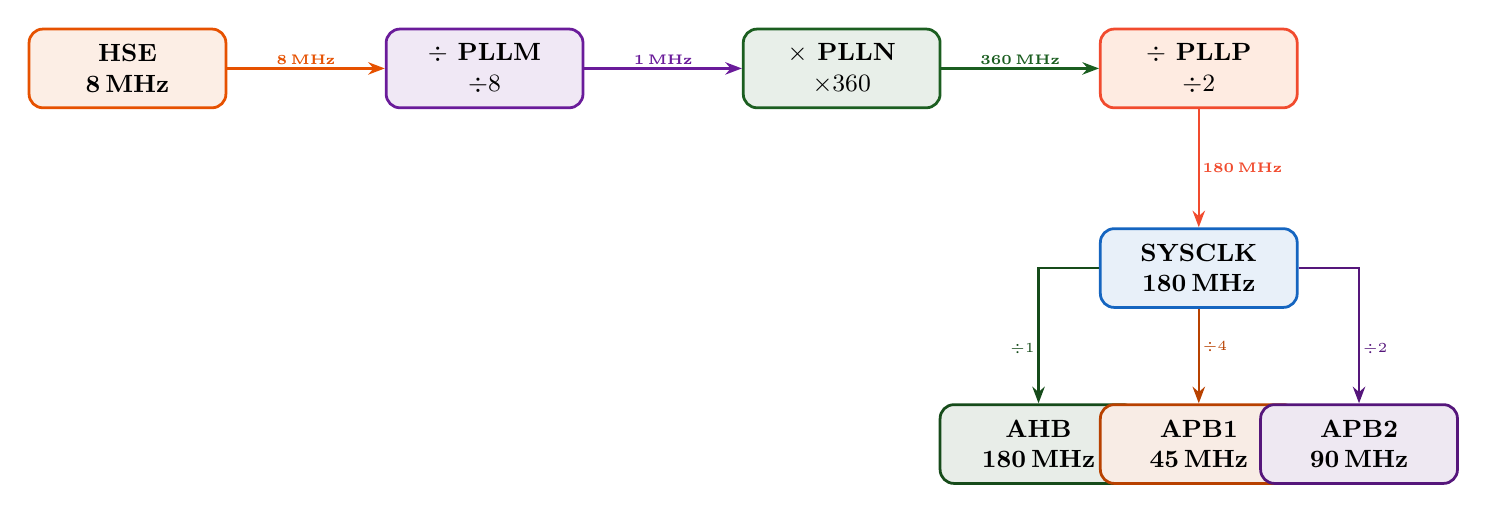
\begin{tikzpicture}[
    block/.style={rectangle, rounded corners=5pt, draw=#1, fill=#1!10, minimum width=2.5cm, minimum height=1cm, align=center, font=\small\bfseries, line width=1pt},
    arr/.style={-{Stealth[length=6pt]}, thick, color=#1},
    lbl/.style={font=\tiny\bfseries, text=#1, fill=white, inner sep=1pt},
]
    \node[block=warnorange] (hse) {HSE\\8\,MHz};
    \node[block=hintpurple, right=2cm of hse] (pllm) {$\div$ PLLM\\$\div 8$};
    \node[block=successgreen, right=2cm of pllm] (plln) {$\times$ PLLN\\$\times 360$};
    \node[block=RedOrange, right=2cm of plln] (pllp) {$\div$ PLLP\\$\div 2$};
    \node[block=accentblue, below=1.5cm of pllp] (sys) {SYSCLK\\180\,MHz};
    
    \node[block=successgreen!80!black, below left=1.2cm and -0.5cm of sys] (ahb) {AHB\\180\,MHz};
    \node[block=warnorange!80!black, below=1.2cm of sys] (apb1) {APB1\\45\,MHz};
    \node[block=hintpurple!80!black, below right=1.2cm and -0.5cm of sys] (apb2) {APB2\\90\,MHz};
    
    \draw[arr=warnorange] (hse) -- node[lbl=warnorange, above] {8\,MHz} (pllm);
    \draw[arr=hintpurple] (pllm) -- node[lbl=hintpurple, above] {1\,MHz} (plln);
    \draw[arr=successgreen] (plln) -- node[lbl=successgreen, above] {360\,MHz} (pllp);
    \draw[arr=RedOrange] (pllp) -- node[lbl=RedOrange, right] {180\,MHz} (sys);
    
    \draw[arr=successgreen!80!black] (sys) -| node[lbl=successgreen!80!black, left, pos=0.8] {$\div 1$} (ahb);
    \draw[arr=warnorange!80!black] (sys) -- node[lbl=warnorange!80!black, right, pos=0.4] {$\div 4$} (apb1);
    \draw[arr=hintpurple!80!black] (sys) -| node[lbl=hintpurple!80!black, right, pos=0.8] {$\div 2$} (apb2);
\end{tikzpicture}
\end{center}

\begin{tipbox}[Key Takeaway]
The I2C1 peripheral sits on the \textbf{APB1 bus at 45\,MHz}. This value is critical because we use it directly when configuring I2C timing (\texttt{CR2 = 45}).
\end{tipbox}

\begin{altbox}[Alternative Implementation]
Instead of using the PLL, you could:
\begin{enumerate}[leftmargin=2em]
    \item \textbf{Use HSI directly (16\,MHz)}: Simpler code, but I2C timing calculations change (\texttt{CR2 = 16}), and USART baud rate divisors change.
    \item \textbf{Use the STM32 HAL library}: Call \texttt{HAL\_RCC\_OscConfig()} and \texttt{HAL\_RCC\_ClockConfig()} --- the HAL calculates everything for you, but you lose understanding of what happens underneath.
\end{enumerate}
\end{altbox}

% ╔══════════════════════════════════════════════════════════════════════════╗
% ║                SECTION 5: GPIO CONFIGURATION                            ║
% ╚══════════════════════════════════════════════════════════════════════════╝
\section{Function: \texttt{GPIO\_CONFIG()} --- Pin Setup}

\subsection{Why Is This Function Needed?}

Every pin on the STM32 is \textbf{multipurpose}. By default, they are just generic input pins. We must \textbf{explicitly configure} each pin for its role:

\begin{itemize}[leftmargin=2em]
    \item \textbf{PA2} $\rightarrow$ USART2 TX (for serial debug output)
    \item \textbf{PB8} $\rightarrow$ I2C1 SCL (clock line)
    \item \textbf{PB9} $\rightarrow$ I2C1 SDA (data line)
\end{itemize}

\subsection{Understanding GPIO Registers}

For each pin, we configure \textbf{five} things:

\begin{center}
\renewcommand{\arraystretch}{1.3}
\begin{tabularx}{\textwidth}{>{\bfseries\color{accentblue}\centering\arraybackslash}p{2.5cm} >{\centering\arraybackslash}p{3.5cm} X}
\toprule
\rowcolor{accentblue!15}
\textbf{Register} & \textbf{What It Controls} & \textbf{Our Setting for I2C Pins} \\
\midrule
MODER & Pin mode (Input/Output/AF/Analog) & \texttt{0b10} = Alternate Function \\
\rowcolor{gray!5}
AFR & Which alternate function (0--15) & AF4 = I2C function \\
OTYPER & Output type (Push-Pull / Open-Drain) & Open-Drain (required for I2C!) \\
\rowcolor{gray!5}
OSPEEDR & Output speed & Medium speed \\
PUPDR & Pull-up / Pull-down & Pull-up (keeps line HIGH when idle) \\
\bottomrule
\end{tabularx}
\end{center}

\subsection{I2C Pin Configuration Code (PB8 --- SCL)}

\begin{codebox}[\faIcon{code}\ \ Configuring PB8 as I2C1 SCL]
\begin{lstlisting}[style=CStyle]
// Step 1: Enable clock for GPIOB
RCC->AHB1ENR |= RCC_AHB1ENR_GPIOBEN;
__NOP(); __NOP(); // Brief delay for clock to stabilize

// Step 2: Set PB8 to Alternate Function mode (0b10)
GPIOB->MODER &= ~(3UL << 8*2);  // Clear bits [17:16]
GPIOB->MODER |=  (2UL << 8*2);  // Set to AF mode

// Step 3: Select AF4 (I2C1) in the Alternate Function Register
//   PB8 is in AFR[1] (high register, pins 8-15)
//   Position = (8-8)*4 = 0, so bits [3:0]
GPIOB->AFR[1] &= ~(0xF << (8-8)*4);  // Clear
GPIOB->AFR[1] |=  (4UL << (8-8)*4);  // AF4 = I2C

// Step 4: Set Open-Drain output (REQUIRED for I2C!)
GPIOB->OTYPER |= (1U << 8);  // 1 = Open-Drain

// Step 5: Set Medium speed
GPIOB->OSPEEDR |= (1U << (8*2));  // 0b01 = Medium

// Step 6: Enable Pull-Up (keeps SCL HIGH when idle)
GPIOB->PUPDR &= ~(3UL << 8*2);  // Clear
GPIOB->PUPDR |=  (1U << (8*2)); // 0b01 = Pull-Up
\end{lstlisting}
\end{codebox}

\begin{warnbox}[Why Open-Drain is Critical for I2C]
I2C uses a \textbf{wired-AND} bus design:
\begin{itemize}[leftmargin=1.5em]
    \item \textbf{Open-Drain} means a pin can only \textit{pull LOW} or \textit{float} (disconnect). It cannot actively drive HIGH.
    \item The \textbf{pull-up resistor} pulls the line HIGH when nobody is pulling it LOW.
    \item This prevents electrical conflict when both master and slave try to control the same line.
    \item If we used \textbf{Push-Pull} instead, the master driving HIGH and slave driving LOW at the same time would cause a \textbf{short circuit}!
\end{itemize}
\end{warnbox}

\begin{altbox}[Alternative Implementation]
\begin{itemize}[leftmargin=1.5em]
    \item \textbf{HAL approach}: \texttt{HAL\_GPIO\_Init(GPIOB, \&GPIO\_InitStruct)} with \texttt{.Mode = GPIO\_MODE\_AF\_OD}, \texttt{.Alternate = GPIO\_AF4\_I2C1}.
    \item \textbf{Different pins}: I2C1 can alternatively use \textbf{PB6} (SCL) and \textbf{PB7} (SDA) instead of PB8/PB9. You would change the MODER/AFR bit positions accordingly.
    \item \textbf{External pull-ups}: Instead of using the MCU's internal pull-ups (\texttildelow40k$\Omega$), you could add external 4.7k$\Omega$ resistors for more reliable communication, especially at higher speeds or with longer wires.
\end{itemize}
\end{altbox}

% ╔══════════════════════════════════════════════════════════════════════════╗
% ║                SECTION 6: USART CONFIGURATION                          ║
% ╚══════════════════════════════════════════════════════════════════════════╝
\section{Function: \texttt{USART2\_CONFIG()} \& \texttt{USART2\_SendString()}}

\subsection{Why Is This Needed?}

USART2 is used for \textbf{debug output}. It sends text to your computer via the Nucleo's built-in USB-to-Serial converter. This is how we see the temperature and pressure readings on a serial terminal (like PuTTY, Tera Term, or the STM32CubeIDE console).

\subsection{Baud Rate Calculation}

\begin{conceptbox}[Baud Rate Math]
The baud rate register (\texttt{BRR}) value is computed as:

\[
\text{USARTDIV} = \frac{f_{\text{APB1}}}{16 \times \text{BaudRate}} = \frac{45{,}000{,}000}{16 \times 115200} \approx 24.414
\]

This is split into:
\begin{itemize}[leftmargin=2em]
    \item \textbf{Mantissa} = 24 (integer part)
    \item \textbf{Fraction} = $0.414 \times 16 \approx 7$ (fractional part, scaled to 4 bits)
\end{itemize}

\texttt{BRR = (24 << 4) | 7 = 0x187} \quad $\Rightarrow$ Actual baud rate $\approx$ 115,108 (close enough to 115,200).
\end{conceptbox}

\begin{codebox}[\faIcon{code}\ \ USART Configuration \& Send Function]
\begin{lstlisting}[style=CStyle]
void USART2_CONFIG(void)
{
    RCC->APB1ENR |= RCC_APB1ENR_USART2EN; // Enable clock
    __NOP();
    USART2->BRR = (24 << 4) | 7;          // 115200 baud
    USART2->CR1 = USART_CR1_TE | USART_CR1_UE; // TX + Enable
}

void USART2_SendString(const char *s)
{
    while (*s) {
        // Wait until transmit buffer is empty
        while (!(USART2->SR & USART_SR_TXE));
        USART2->DR = (uint8_t)(*s++); // Send one character
    }
    // Wait until transmission is complete
    while (!(USART2->SR & USART_SR_TC));
}
\end{lstlisting}
\end{codebox}

% ╔══════════════════════════════════════════════════════════════════════════╗
% ║                SECTION 7: TIMER & DELAY                                 ║
% ╚══════════════════════════════════════════════════════════════════════════╝
\section{Functions: \texttt{TIM6\_CONFIG()}, \texttt{delay\_us()}, \texttt{delay\_ms()}}

\subsection{Why Are These Needed?}

The BMP280 sensor requires \textbf{precise timing delays} during initialization (e.g., waiting after a soft reset). The code uses \textbf{TIM6}, a basic hardware timer, to create microsecond-accurate delays.

\begin{codebox}[\faIcon{code}\ \ Timer Setup \& Delay Functions]
\begin{lstlisting}[style=CStyle]
void TIM6_CONFIG(void)
{
    RCC->APB1ENR |= RCC_APB1ENR_TIM6EN; // Enable TIM6 clock
    TIM6->PSC = 89U;       // 90MHz / (89+1) = 1MHz -> 1 tick = 1us
    TIM6->ARR = 0xFFFFU;   // Count up to 65535 (free-running)
    TIM6->EGR = TIM_EGR_UG; // Load PSC/ARR immediately
    TIM6->CR1 |= TIM_CR1_CEN; // Start counting
}

void delay_us(uint16_t us)
{
    TIM6->CNT = 0U;                  // Reset counter to 0
    while ((uint16_t)TIM6->CNT < us); // Wait until count reaches 'us'
}

void delay_ms(uint32_t ms)
{
    for (uint32_t i = 0; i < ms; i++)
        delay_us(1000U);  // 1000 microseconds = 1 millisecond
}
\end{lstlisting}
\end{codebox}

\begin{tipbox}[Timer Math]
TIM6 is on APB1 (45\,MHz), but since the APB1 prescaler is $\div 4$ (not $\div 1$), the timer clock is actually \textbf{$45 \times 2 = 90$\,MHz} (timers on APB1 get $\times 2$ when the APB prescaler $> 1$).

With \texttt{PSC = 89}: frequency = $90\text{\,MHz} / (89+1) = 1\text{\,MHz}$, so each tick = $1\,\mu s$.
\end{tipbox}

\begin{altbox}[Alternative Delay Approaches]
\begin{enumerate}[leftmargin=2em]
    \item \textbf{SysTick timer}: ARM Cortex-M4 has a built-in SysTick timer --- simpler for delays but less flexible.
    \item \textbf{HAL\_Delay()}: The HAL library provides \texttt{HAL\_Delay(ms)} using SysTick interrupt.
    \item \textbf{Software loop delay}: Simple \texttt{for} loop counting cycles. Unreliable because compiler optimizations can change the timing.
    \item \textbf{DWT cycle counter}: The Debug Watchpoint and Trace unit has a cycle counter (\texttt{DWT->CYCCNT}) for nanosecond-precision delays.
\end{enumerate}
\end{altbox}

% ╔══════════════════════════════════════════════════════════════════════════╗
% ║                SECTION 8: I2C CONFIGURATION                             ║
% ╚══════════════════════════════════════════════════════════════════════════╝
\section{Function: \texttt{I2C\_CONFIG()} --- The Heart of I2C Setup}

\subsection{Why Is This Function Needed?}

This function initializes the STM32's I2C1 peripheral hardware. Without this, the I2C hardware block is dormant and cannot generate clock signals or send/receive data.

\begin{codebox}[\faIcon{code}\ \ I2C\_CONFIG() --- Full Code with Detailed Comments]
\begin{lstlisting}[style=CStyle]
void I2C_CONFIG(void)
{
    // 1. Enable I2C1 peripheral clock
    RCC->APB1ENR |= RCC_APB1ENR_I2C1EN;

    // 2. Reset the I2C peripheral (ensures clean state)
    RCC->APB1RSTR |= RCC_APB1RSTR_I2C1RST;   // Assert reset
    RCC->APB1RSTR &= ~RCC_APB1RSTR_I2C1RST;   // Release reset

    // 3. Set peripheral input clock frequency (APB1 = 45MHz)
    I2C1->CR2 = 45U;

    // 4. Set Clock Control Register for 100kHz (Standard Mode)
    //    CCR = APB1_freq / (2 * I2C_freq)
    //        = 45,000,000 / (2 * 100,000) = 225
    I2C1->CCR = 225U;

    // 5. Set maximum rise time
    //    TRISE = (APB1_freq_MHz * max_rise_time_us) + 1
    //          = (45 * 1) + 1 = 46
    I2C1->TRISE = 46U;

    // 6. Enable the I2C peripheral
    I2C1->CR1 |= I2C_CR1_PE;
}
\end{lstlisting}
\end{codebox}

\subsection{Understanding Each Register}

\begin{registerbox}[I2C Register Details]
\renewcommand{\arraystretch}{1.4}
\begin{tabularx}{\textwidth}{>{\ttfamily\bfseries\color{deepblue}}p{2cm} >{\centering\arraybackslash}p{2.5cm} X}
\toprule
\rowcolor{warnorange!15}
\textbf{Register} & \textbf{Value} & \textbf{Explanation} \\
\midrule
CR2 & 45 & Tells the I2C hardware ``my input clock is 45\,MHz.'' It needs this to calculate timing. \\
\rowcolor{gray!5}
CCR & 225 & Clock Control Register. For standard mode (100\,kHz), each half-period of SCL = $225 / 45\text{\,MHz} = 5\,\mu s$. Full period = $10\,\mu s = 100\text{\,kHz}$. \\
TRISE & 46 & Maximum allowed rise time. For standard mode, the I2C spec says $\leq 1000\,\text{ns}$. Formula: $(45 \times 1) + 1 = 46$. \\
\rowcolor{gray!5}
CR1 & PE bit & Peripheral Enable --- turns on the I2C hardware. \\
\bottomrule
\end{tabularx}
\end{registerbox}

\begin{conceptbox}[CCR Calculation Deep Dive]
For \textbf{Standard Mode (Sm)} at 100\,kHz:
\[
\text{CCR} = \frac{f_{\text{APB1}}}{2 \times f_{\text{I2C}}} = \frac{45{,}000{,}000}{2 \times 100{,}000} = 225
\]

For \textbf{Fast Mode (Fm)} at 400\,kHz with 2:1 duty cycle:
\[
\text{CCR} = \frac{f_{\text{APB1}}}{3 \times f_{\text{I2C}}} = \frac{45{,}000{,}000}{3 \times 400{,}000} = 37.5 \approx 38
\]
(You would also set the \texttt{F/S} bit and \texttt{DUTY} bit in CCR for Fast Mode.)
\end{conceptbox}

\begin{altbox}[Alternative I2C Configuration Approaches]
\begin{itemize}[leftmargin=1.5em]
    \item \textbf{Fast Mode (400\,kHz)}: Set \texttt{CCR |= I2C\_CCR\_FS} and recalculate CCR. Faster but needs better pull-ups.
    \item \textbf{HAL Library}: \texttt{HAL\_I2C\_Init(\&hi2c1)} with \texttt{.ClockSpeed = 100000} handles all math for you.
    \item \textbf{I2C2 or I2C3}: The STM32F446 has three I2C peripherals. You could use I2C2 (PB10/PB11) or I2C3 (PA8/PC9) with the same logic, just changing the peripheral base address and pins.
    \item \textbf{DMA-based I2C}: For large data transfers, you could configure DMA to handle I2C reads/writes without CPU involvement.
\end{itemize}
\end{altbox}

% ╔══════════════════════════════════════════════════════════════════════════╗
% ║                SECTION 9: I2C WRITE BYTE                                ║
% ╚══════════════════════════════════════════════════════════════════════════╝
\section{Function: \texttt{I2C\_WRITE\_BYTE()} --- Writing to the Sensor}

\subsection{Why Is This Function Needed?}

To control the BMP280, we need to \textbf{write values into its registers}. For example:
\begin{itemize}[leftmargin=2em]
    \item Write \texttt{0xB6} to register \texttt{0xE0} to reset the sensor
    \item Write \texttt{0x57} to register \texttt{0xF4} to start measurements
\end{itemize}

\subsection{I2C Write Transaction Diagram}

\begin{center}
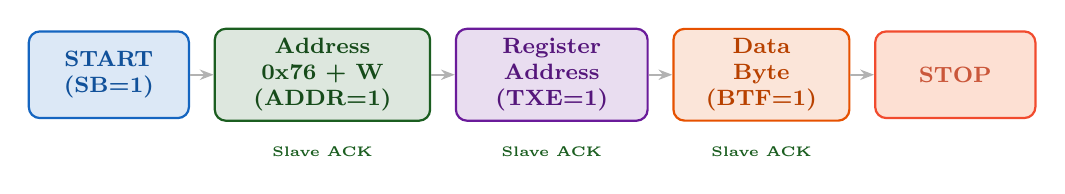
\begin{tikzpicture}[
    phase/.style={rectangle, rounded corners=4pt, draw=#1, fill=#1!15, minimum height=1.1cm, align=center, font=\footnotesize\bfseries, text=#1!80!black, line width=0.8pt},
    arr/.style={-{Stealth[length=5pt]}, thick, color=gray!60},
]
    \node[phase=accentblue, text width=1.8cm] (start) {START\\(SB=1)};
    \node[phase=successgreen, text width=2.5cm, right=0.3cm of start] (addr) {Address\\0x76 + W\\(ADDR=1)};
    \node[phase=hintpurple, text width=2.2cm, right=0.3cm of addr] (reg) {Register\\Address\\(TXE=1)};
    \node[phase=warnorange, text width=2cm, right=0.3cm of reg] (data) {Data\\Byte\\(BTF=1)};
    \node[phase=RedOrange, text width=1.8cm, right=0.3cm of data] (stop) {STOP};
    
    \draw[arr] (start) -- (addr);
    \draw[arr] (addr) -- (reg);
    \draw[arr] (reg) -- (data);
    \draw[arr] (data) -- (stop);
    
    % ACK indicators
    \node[font=\tiny\bfseries, text=successgreen, below=0.2cm of addr] {Slave ACK};
    \node[font=\tiny\bfseries, text=successgreen, below=0.2cm of reg] {Slave ACK};
    \node[font=\tiny\bfseries, text=successgreen, below=0.2cm of data] {Slave ACK};
\end{tikzpicture}
\end{center}

\begin{codebox}[\faIcon{code}\ \ I2C\_WRITE\_BYTE() --- Annotated]
\begin{lstlisting}[style=CStyle]
void I2C_WRITE_BYTE(uint8_t reg, uint8_t data)
{
    // Phase 1: Generate START condition on the bus
    I2C1->CR1 |= I2C_CR1_START;
    while (!(I2C1->SR1 & I2C_SR1_SB)); // Wait for SB (Start Bit) flag

    // Phase 2: Send slave address (0x76) with WRITE bit (LSB = 0)
    //   Address on wire = 0x76 << 1 | 0 = 0xEC
    I2C1->DR = (BME_P280_I2C_ADDRESS << 1) | 0;
    while (!(I2C1->SR1 & I2C_SR1_ADDR)); // Wait for ADDR flag (slave ACK'd)
    (void)I2C1->SR2; // MUST read SR2 to clear ADDR flag (hardware requirement)

    // Phase 3: Send the register address (e.g., 0xF4 for ctrl_meas)
    I2C1->DR = reg;
    while (!(I2C1->SR1 & I2C_SR1_TXE)); // Wait for TX buffer empty

    // Phase 4: Send the data byte (e.g., 0x57)
    I2C1->DR = data;
    while (!(I2C1->SR1 & I2C_SR1_BTF)); // Wait for Byte Transfer Finished

    // Phase 5: Generate STOP condition
    I2C1->CR1 |= I2C_CR1_STOP;
}
\end{lstlisting}
\end{codebox}

\begin{warnbox}[Why Read SR2 to Clear ADDR?]
This is an STM32 hardware quirk! The ADDR flag is cleared by a \textbf{specific sequence}: read SR1 (done by the \texttt{while} loop) then read SR2. The \texttt{(void)I2C1->SR2;} cast tells the compiler ``I'm reading this on purpose, don't optimize it away.'' If you forget this step, the I2C will hang!
\end{warnbox}

\begin{altbox}[Alternative Write Approaches]
\begin{itemize}[leftmargin=1.5em]
    \item \textbf{HAL Library}: \texttt{HAL\_I2C\_Mem\_Write(\&hi2c1, 0x76<<1, reg, I2C\_MEMADD\_SIZE\_8BIT, \&data, 1, 100);}
    \item \textbf{Interrupt-driven}: Instead of polling flags in \texttt{while} loops, you could use I2C event interrupts (\texttt{I2C1\_EV\_IRQHandler}) for non-blocking writes.
    \item \textbf{DMA-driven}: For writing many bytes, configure DMA to feed bytes automatically without CPU intervention.
\end{itemize}
\end{altbox}

% ╔══════════════════════════════════════════════════════════════════════════╗
% ║                SECTION 10: I2C READ BYTE                                ║
% ╚══════════════════════════════════════════════════════════════════════════╝
\section{Function: \texttt{I2C\_READ\_BYTE()} --- Reading a Single Byte}

\subsection{Why Is This Needed?}

Reading from the BMP280 is a \textbf{two-phase process}:
\begin{enumerate}[leftmargin=2em]
    \item \textbf{Write phase}: Tell the sensor \textit{which register} you want to read (e.g., chip ID at \texttt{0xD0})
    \item \textbf{Read phase}: Switch direction and read the data back
\end{enumerate}

This requires a \textbf{Repeated START} --- instead of STOP then START, you send another START without releasing the bus.

\subsection{I2C Read Transaction Diagram}

\begin{center}
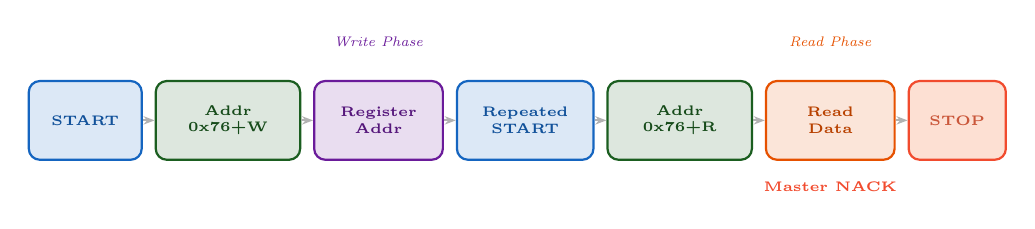
\begin{tikzpicture}[
    phase/.style={rectangle, rounded corners=4pt, draw=#1, fill=#1!15, minimum height=1cm, align=center, font=\tiny\bfseries, text=#1!80!black, line width=0.8pt},
    arr/.style={-{Stealth[length=4pt]}, thick, color=gray!60},
]
    \node[phase=accentblue, text width=1.2cm] (s1) {START};
    \node[phase=successgreen, text width=1.6cm, right=0.15cm of s1] (a1) {Addr\\0x76+W};
    \node[phase=hintpurple, text width=1.4cm, right=0.15cm of a1] (reg) {Register\\Addr};
    \node[phase=accentblue, text width=1.5cm, right=0.15cm of reg] (sr) {Repeated\\START};
    \node[phase=successgreen, text width=1.6cm, right=0.15cm of sr] (a2) {Addr\\0x76+R};
    \node[phase=warnorange, text width=1.4cm, right=0.15cm of a2] (data) {Read\\Data};
    \node[phase=RedOrange, text width=1cm, right=0.15cm of data] (stop) {STOP};
    
    \draw[arr] (s1) -- (a1);
    \draw[arr] (a1) -- (reg);
    \draw[arr] (reg) -- (sr);
    \draw[arr] (sr) -- (a2);
    \draw[arr] (a2) -- (data);
    \draw[arr] (data) -- (stop);
    
    % Labels
    \node[font=\tiny\itshape, text=hintpurple, above=0.3cm of reg] {Write Phase};
    \node[font=\tiny\itshape, text=warnorange, above=0.3cm of data] {Read Phase};
    
    % NACK label
    \node[font=\tiny\bfseries, text=RedOrange, below=0.15cm of data] {Master NACK};
\end{tikzpicture}
\end{center}

\begin{codebox}[\faIcon{code}\ \ I2C\_READ\_BYTE() --- Annotated]
\begin{lstlisting}[style=CStyle]
uint8_t I2C_READ_BYTE(uint8_t reg)
{
    uint8_t val = 0xFF;

    // === WRITE PHASE: Tell sensor which register to read ===
    I2C1->CR1 |= I2C_CR1_START;                    // START
    while (!(I2C1->SR1 & I2C_SR1_SB));

    I2C1->DR = (BME_P280_I2C_ADDRESS << 1) | 0;    // Address + WRITE
    while (!(I2C1->SR1 & I2C_SR1_ADDR));
    (void)I2C1->SR2;

    I2C1->DR = reg;                                  // Register address
    while (!(I2C1->SR1 & I2C_SR1_BTF));

    // === READ PHASE: Repeated START + read data ===
    I2C1->CR1 |= I2C_CR1_START;                     // Repeated START
    while (!(I2C1->SR1 & I2C_SR1_SB));

    I2C1->CR1 &= ~I2C_CR1_ACK;  // NACK (only reading 1 byte)
    I2C1->DR = (BME_P280_I2C_ADDRESS << 1) | 1;     // Address + READ
    while (!(I2C1->SR1 & I2C_SR1_ADDR));
    (void)I2C1->SR2;

    I2C1->CR1 |= I2C_CR1_STOP;                      // Queue STOP
    while (!(I2C1->SR1 & I2C_SR1_RXNE));             // Wait for data

    val = (uint8_t)I2C1->DR;                         // Read the byte
    return val;
}
\end{lstlisting}
\end{codebox}

\begin{conceptbox}[Why NACK Before the Last Byte?]
In I2C protocol:
\begin{itemize}[leftmargin=1.5em]
    \item \textbf{ACK} (Acknowledge) means ``I received the byte, \textit{send me more}.''
    \item \textbf{NACK} (Not Acknowledge) means ``I received the byte, \textit{stop sending}.''
\end{itemize}
When reading only 1 byte, the master must send \textbf{NACK immediately} to tell the slave ``don't send any more data.'' If you forget to clear the ACK flag, the slave will keep sending bytes, causing data corruption!
\end{conceptbox}

% ╔══════════════════════════════════════════════════════════════════════════╗
% ║                SECTION 11: I2C READ BYTES (BURST)                       ║
% ╚══════════════════════════════════════════════════════════════════════════╝
\section{Function: \texttt{I2C\_READ\_BYTES()} --- Multi-Byte Burst Read}

\subsection{Why Is This Needed?}

The BMP280 calibration data spans \textbf{24 consecutive registers} (0x88--0x9F), and raw sensor data spans \textbf{8 registers} (0xF7--0xFE). Reading them one by one would be extremely slow. \textbf{Burst read} reads all of them in a single I2C transaction.

\begin{tipbox}[How Burst Read Works]
The BMP280 has an \textbf{auto-increment} feature: once you send the starting register address, the sensor automatically advances its internal pointer to the next register after each byte. So you just keep reading!
\end{tipbox}

\begin{codebox}[\faIcon{code}\ \ I2C\_READ\_BYTES() --- Multi-byte Read]
\begin{lstlisting}[style=CStyle]
void I2C_READ_BYTES(uint8_t start_reg, uint8_t *buf, uint8_t len)
{
    if (len == 0) return;

    // WRITE PHASE: Send the starting register address
    I2C1->CR1 |= I2C_CR1_START;
    while (!(I2C1->SR1 & I2C_SR1_SB));

    I2C1->DR = (BME_P280_I2C_ADDRESS << 1) | 0;  // Address + WRITE
    while (!(I2C1->SR1 & I2C_SR1_ADDR));
    (void)I2C1->SR2;

    I2C1->DR = start_reg;                         // Starting register
    while (!(I2C1->SR1 & I2C_SR1_BTF));

    // READ PHASE: Repeated START + read multiple bytes
    I2C1->CR1 |= I2C_CR1_START;
    while (!(I2C1->SR1 & I2C_SR1_SB));

    I2C1->CR1 |= I2C_CR1_ACK;  // Enable ACK (we want multiple bytes)
    I2C1->DR = (BME_P280_I2C_ADDRESS << 1) | 1;   // Address + READ
    while (!(I2C1->SR1 & I2C_SR1_ADDR));
    (void)I2C1->SR2;

    // Read loop
    for (uint8_t i = 0; i < len; i++)
    {
        if (i == (len - 1))
        {
            I2C1->CR1 &= ~I2C_CR1_ACK;   // NACK for last byte
            I2C1->CR1 |= I2C_CR1_STOP;    // Generate STOP
        }
        while (!(I2C1->SR1 & I2C_SR1_RXNE)); // Wait for data
        buf[i] = (uint8_t)I2C1->DR;           // Store byte
    }
}
\end{lstlisting}
\end{codebox}

\begin{conceptbox}[ACK/NACK Strategy for Multi-Byte Reads]
\begin{center}
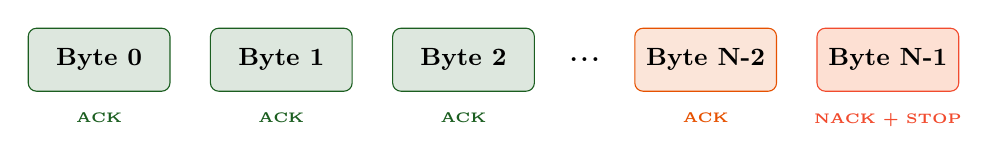
\begin{tikzpicture}[
    byte/.style={rectangle, rounded corners=3pt, draw=#1, fill=#1!15, minimum width=1.8cm, minimum height=0.8cm, align=center, font=\small\bfseries},
]
    \node[byte=successgreen] (b1) {Byte 0};
    \node[byte=successgreen, right=0.5cm of b1] (b2) {Byte 1};
    \node[byte=successgreen, right=0.5cm of b2] (b3) {Byte 2};
    \node[font=\Large, right=0.3cm of b3] (dots) {...};
    \node[byte=warnorange, right=0.3cm of dots] (bn1) {Byte N-2};
    \node[byte=RedOrange, right=0.5cm of bn1] (bn) {Byte N-1};
    
    \node[font=\tiny\bfseries, text=successgreen, below=0.15cm of b1] {ACK};
    \node[font=\tiny\bfseries, text=successgreen, below=0.15cm of b2] {ACK};
    \node[font=\tiny\bfseries, text=successgreen, below=0.15cm of b3] {ACK};
    \node[font=\tiny\bfseries, text=warnorange, below=0.15cm of bn1] {ACK};
    \node[font=\tiny\bfseries, text=RedOrange, below=0.15cm of bn] {\textbf{NACK + STOP}};
\end{tikzpicture}
\end{center}

\begin{itemize}[leftmargin=1.5em]
    \item Send \textbf{ACK} after every byte \textit{except} the last one $\rightarrow$ tells slave ``keep going''
    \item Send \textbf{NACK + STOP} after the last byte $\rightarrow$ tells slave ``we're done''
\end{itemize}
\end{conceptbox}

% ╔══════════════════════════════════════════════════════════════════════════╗
% ║                SECTION 12: I2C DEVICE ALIVE                             ║
% ╚══════════════════════════════════════════════════════════════════════════╝
\section{Function: \texttt{I2C\_DEVICE\_ALIVE()} --- Connection Check}

\subsection{Why Is This Needed?}

Before trying to read data, we need to verify the BMP280 is \textbf{actually connected and responding}. This function sends just the address and checks if the slave responds with ACK.

\begin{codebox}[\faIcon{code}\ \ I2C\_DEVICE\_ALIVE() --- Connection Probe]
\begin{lstlisting}[style=CStyle]
int I2C_DEVICE_ALIVE(void)
{
    I2C1->CR1 |= I2C_CR1_START;           // START
    while (!(I2C1->SR1 & I2C_SR1_SB));

    I2C1->DR = (BME_P280_I2C_ADDRESS << 1) | 0;  // Address + WRITE

    uint32_t timeout = 200000;
    // Wait for either ADDR (ACK) or AF (NACK/no response)
    while (!(I2C1->SR1 & (I2C_SR1_ADDR | I2C_SR1_AF)) && --timeout);

    int alive = (I2C1->SR1 & I2C_SR1_ADDR) != 0;  // Check if ACK'd
    if (alive)
        (void)I2C1->SR2;          // Clear ADDR flag
    else
        I2C1->SR1 &= ~I2C_SR1_AF; // Clear AF (Acknowledge Failure) flag

    I2C1->CR1 |= I2C_CR1_STOP;
    delay_ms(2);
    return alive;  // 1 = alive, 0 = not responding
}
\end{lstlisting}
\end{codebox}

\begin{conceptbox}[Understanding ADDR vs AF Flags]
\begin{center}
\renewcommand{\arraystretch}{1.3}
\begin{tabularx}{\textwidth}{>{\centering\bfseries\color{accentblue}}p{2cm} >{\centering}p{4cm} X}
\toprule
\rowcolor{accentblue!15}
\textbf{Flag} & \textbf{Full Name} & \textbf{Meaning} \\
\midrule
ADDR & Address Sent/Matched & The slave \textit{responded} with an ACK $\rightarrow$ device is alive! \\
\rowcolor{gray!5}
AF & Acknowledge Failure & No slave responded (NACK) $\rightarrow$ device not connected or wrong address. \\
\bottomrule
\end{tabularx}
\end{center}
\end{conceptbox}

\begin{altbox}[Alternative Alive-Check Approaches]
\begin{itemize}[leftmargin=1.5em]
    \item \textbf{Read Chip ID}: Instead of just checking ACK, read the chip ID register (\texttt{0xD0}). If you get \texttt{0x58} (BMP280), the device is definitely alive and correct.
    \item \textbf{I2C Bus Scanner}: Loop through all 127 possible addresses and check which ones ACK. Useful for debugging when you don't know the sensor's address.
    \item \textbf{HAL}: \texttt{HAL\_I2C\_IsDeviceReady(\&hi2c1, 0x76 << 1, 3, 100)} tries 3 times with 100\,ms timeout.
\end{itemize}
\end{altbox}

% ╔══════════════════════════════════════════════════════════════════════════╗
% ║                SECTION 13: CALIBRATION                                  ║
% ╚══════════════════════════════════════════════════════════════════════════╝
\section{Function: \texttt{BME\_P280\_CALIBRATION\_READ()}}

\subsection{Why Are Calibration Values Needed?}

Every BMP280 chip is \textbf{slightly different} due to manufacturing variations. Bosch stores \textbf{factory calibration coefficients} inside each sensor's non-volatile memory. These numbers are used in compensation formulas to convert raw ADC readings into accurate temperature and pressure values.

\begin{conceptbox}[Calibration Structure]
The calibration data is organized into three groups:

\begin{center}
\renewcommand{\arraystretch}{1.3}
\begin{tabularx}{\textwidth}{>{\bfseries\color{accentblue}}p{2.5cm} >{\centering\arraybackslash}p{3cm} >{\centering\arraybackslash}p{2.5cm} X}
\toprule
\rowcolor{accentblue!15}
\textbf{Group} & \textbf{Coefficients} & \textbf{Register Range} & \textbf{Data Type} \\
\midrule
Temperature & TEMP\_1, 2, 3 & 0x88--0x8D & uint16, int16, int16 \\
\rowcolor{gray!5}
Pressure & PRESS\_1 -- 9 & 0x8E--0x9F & uint16 + 8$\times$int16 \\
Humidity & HUM\_1 -- 6 & 0xA1 + 0xE1--0xE7 & Mixed types \\
\bottomrule
\end{tabularx}
\end{center}
\end{conceptbox}

\begin{codebox}[\faIcon{code}\ \ Calibration Read (Temperature \& Pressure)]
\begin{lstlisting}[style=CStyle]
void BME_P280_CALIBRATION_READ(void)
{
    uint8_t CALIB_VAL[24];
    // Read 24 consecutive bytes starting at 0x88
    I2C_READ_BYTES(BME_P280_REGISTER_CALIBRATION_START, CALIB_VAL, 24);

    // Temperature calibration (bytes 0-5)
    //  Each parameter is 16-bit, stored LSB first (little-endian)
    CALIBRATION.TEMP_1 = (uint16_t)((CALIB_VAL[1] << 8) | CALIB_VAL[0]);
    CALIBRATION.TEMP_2 = (int16_t) ((CALIB_VAL[3] << 8) | CALIB_VAL[2]);
    CALIBRATION.TEMP_3 = (int16_t) ((CALIB_VAL[5] << 8) | CALIB_VAL[4]);

    // Pressure calibration (bytes 6-23)
    CALIBRATION.PRESS_1 = (uint16_t)((CALIB_VAL[7]  << 8) | CALIB_VAL[6]);
    CALIBRATION.PRESS_2 = (int16_t) ((CALIB_VAL[9]  << 8) | CALIB_VAL[8]);
    // ... PRESS_3 through PRESS_9 follow the same pattern ...
    CALIBRATION.PRESS_9 = (int16_t) ((CALIB_VAL[23] << 8) | CALIB_VAL[22]);
}
\end{lstlisting}
\end{codebox}

\begin{tipbox}[Little-Endian Byte Order]
The BMP280 stores multi-byte values in \textbf{little-endian} format: the \textbf{least significant byte (LSB) comes first}. That's why we see:
\begin{center}
\texttt{value = (HIGH\_BYTE << 8) | LOW\_BYTE}
\end{center}
For example, if register 0x88 = \texttt{0x34} and 0x89 = \texttt{0x12}, then TEMP\_1 = \texttt{0x1234}.
\end{tipbox}

% ╔══════════════════════════════════════════════════════════════════════════╗
% ║                SECTION 14: SENSOR INIT                                  ║
% ╚══════════════════════════════════════════════════════════════════════════╝
\section{Function: \texttt{BME\_P280\_INIT()} --- Sensor Initialization}

\begin{codebox}[\faIcon{code}\ \ BME\_P280\_INIT() --- Step-by-Step Initialization]
\begin{lstlisting}[style=CStyle]
void BME_P280_INIT(void)
{
    // Step 1: Soft-reset the sensor
    //   Writing 0xB6 to the reset register (0xE0)
    //   resets all internal registers to defaults
    I2C_WRITE_BYTE(BME_P280_REGISTER_RESET, BME_P280_RESET_VALUE);
    delay_ms(10); // Sensor needs ~2ms to reset, we give it 10ms

    // Step 2: Set the config register (0xF5)
    //   Value 0x90 = IIR filter x16, standby time 125ms
    I2C_WRITE_BYTE(BME_P280_REGISTER_CONFIGURE, BME_P280_CONFIGURE_VALUE);
    delay_ms(2);

    // Step 3: (BME280 only) Set humidity oversampling
    I2C_WRITE_BYTE(BME_P280_REGISTER_CTRL_HUM, BME_P280_CTRL_HUM_VALUE);
    delay_ms(2);

    // Step 4: Set measurement control (0xF4)
    //   Value 0x57 = Temp x2, Pressure x16, Normal mode
    //   IMPORTANT: ctrl_meas must be written AFTER ctrl_hum!
    I2C_WRITE_BYTE(BME_P280_REGISTER_CONTROL_MEASURE,
                    BME_P280_CONTROL_MEASURE_VALUE);
    delay_ms(2);
}
\end{lstlisting}
\end{codebox}

\begin{warnbox}[Register Write Order Matters!]
According to the Bosch datasheet:
\begin{itemize}[leftmargin=1.5em]
    \item \texttt{config} (0xF5) should be written \textbf{before} entering Normal mode
    \item \texttt{ctrl\_hum} (0xF2) must be written \textbf{before} \texttt{ctrl\_meas} (0xF4) --- the humidity settings only take effect when \texttt{ctrl\_meas} is written
\end{itemize}
If you write them in the wrong order, the sensor may use old/default settings!
\end{warnbox}

\begin{conceptbox}[IIR Filter Explained (Config Register 0xF5)]
The BMP280 has a built-in \textbf{IIR (Infinite Impulse Response) filter} that smooths out pressure readings by averaging with previous measurements:

\[
\text{filtered} = \frac{(\text{coefficient} - 1) \times \text{previous} + \text{new}}{\text{coefficient}}
\]

Our code sets coefficient = 16 (high filtering), which eliminates short-term fluctuations like door slams or wind gusts. For weather monitoring, this is ideal. For altitude tracking in a drone, you might want coefficient = 2 (faster response).
\end{conceptbox}

% ╔══════════════════════════════════════════════════════════════════════════╗
% ║                SECTION 15: COMPENSATION FORMULAS                        ║
% ╚══════════════════════════════════════════════════════════════════════════╝
\section{Compensation Functions --- Converting Raw Data to Real Values}

\subsection{Why Compensation Is Needed}

The BMP280's ADC gives \textbf{raw 20-bit numbers} that don't directly represent temperature or pressure. Bosch provides \textbf{fixed-point integer compensation formulas} (no floating-point!) that use the calibration coefficients to convert these raw values.

\subsection{Temperature Compensation}

\begin{codebox}[\faIcon{code}\ \ BME\_P280\_BOSCH\_TEMP\_COMPENSATE()]
\begin{lstlisting}[style=CStyle]
int32_t BME_P280_BOSCH_TEMP_COMPENSATE(int32_t adc_T)
{
    int32_t var1, var2, T;

    // Linear correction term
    var1 = ((((adc_T >> 3) - ((int32_t)CALIBRATION.TEMP_1 << 1)))
             * ((int32_t)CALIBRATION.TEMP_2)) >> 11;

    // Quadratic correction term (handles non-linearity)
    var2 = (((((adc_T >> 4) - ((int32_t)CALIBRATION.TEMP_1))
             * ((adc_T >> 4) - ((int32_t)CALIBRATION.TEMP_1))) >> 12)
             * ((int32_t)CALIBRATION.TEMP_3)) >> 14;

    // t_fine: a global variable shared with pressure/humidity formulas
    t_fine = var1 + var2;

    // Temperature in units of 0.01 degrees Celsius
    T = (t_fine * 5 + 128) >> 8;

    return T;  // e.g., 2534 means 25.34 degrees C
}
\end{lstlisting}
\end{codebox}

\begin{conceptbox}[Understanding \texttt{t\_fine}]
The variable \texttt{t\_fine} is the \textbf{most important intermediate value}. It represents a ``fine temperature'' that captures the sensor's current thermal state. Both the \textbf{pressure} and \textbf{humidity} compensation formulas use \texttt{t\_fine} because:

\begin{itemize}[leftmargin=1.5em]
    \item Pressure measurements are \textit{temperature-dependent} (warm air is less dense)
    \item Humidity readings drift with temperature
\end{itemize}

\textbf{Temperature must ALWAYS be compensated first}, so that \texttt{t\_fine} is available for the other formulas.
\end{conceptbox}

\begin{tipbox}[Fixed-Point Arithmetic]
The formulas use \textbf{bit shifts} instead of division (\texttt{>> 8} instead of \texttt{/ 256}) because:
\begin{itemize}[leftmargin=1.5em]
    \item STM32F4 has no floating-point division unit for 64-bit types
    \item Integer arithmetic is \textbf{deterministic} --- no rounding errors
    \item Bit shifts execute in \textbf{1 clock cycle} vs. division which takes 2--12 cycles
\end{itemize}
The final result is in \textbf{hundredths of a degree}: 2534 = 25.34$^\circ$C.
\end{tipbox}

\subsection{Pressure Compensation}

\begin{codebox}[\faIcon{code}\ \ BME\_P280\_BOSCH\_PRESS\_COMPENSATE() --- Key Steps]
\begin{lstlisting}[style=CStyle]
uint32_t BME_P280_BOSCH_PRESS_COMPENSATE(int32_t adc_P)
{
    int64_t var1, var2, p;

    var1 = ((int64_t)t_fine) - 128000;  // Temperature correction base

    // Higher-order polynomial corrections using PRESS_2 through PRESS_6
    var2 = var1 * var1 * (int64_t)CALIBRATION.PRESS_6;
    var2 = var2 + ((var1 * (int64_t)CALIBRATION.PRESS_5) << 17);
    var2 = var2 + (((int64_t)CALIBRATION.PRESS_4) << 35);

    var1 = ((var1 * var1 * (int64_t)CALIBRATION.PRESS_3) >> 8)
         + ((var1 * (int64_t)CALIBRATION.PRESS_2) << 12);
    var1 = (((((int64_t)1) << 47) + var1))
         * ((int64_t)CALIBRATION.PRESS_1) >> 33;

    if (var1 == 0) return 0;  // Guard: avoid division by zero

    p = 1048576 - adc_P;
    p = (((p << 31) - var2) * 3125) / var1;

    // Final corrections using PRESS_7, PRESS_8, PRESS_9
    var1 = (((int64_t)CALIBRATION.PRESS_9) * (p >> 13) * (p >> 13)) >> 25;
    var2 = (((int64_t)CALIBRATION.PRESS_8) * p) >> 19;
    p = ((p + var1 + var2) >> 8) + (((int64_t)CALIBRATION.PRESS_7) << 4);

    return (uint32_t)(p >> 8);  // Pressure in Pascals
}
\end{lstlisting}
\end{codebox}

\begin{tipbox}[Pressure Units]
\begin{itemize}[leftmargin=1.5em]
    \item The function returns pressure in \textbf{Pascals (Pa)}
    \item Standard atmospheric pressure = 101325\,Pa = 1013.25\,hPa
    \item The code divides by 100 later to display in \textbf{hectopascals (hPa)}, which is the standard meteorological unit
\end{itemize}
\end{tipbox}

% ╔══════════════════════════════════════════════════════════════════════════╗
% ║                SECTION 16: READING AND DISPLAYING                       ║
% ╚══════════════════════════════════════════════════════════════════════════╝
\section{Function: \texttt{BME\_P280\_TEMP\_PRESS\_HUM()}}

\subsection{How Raw Data Is Structured}

Reading 8 bytes starting from \texttt{0xF7} gives us:

\begin{center}
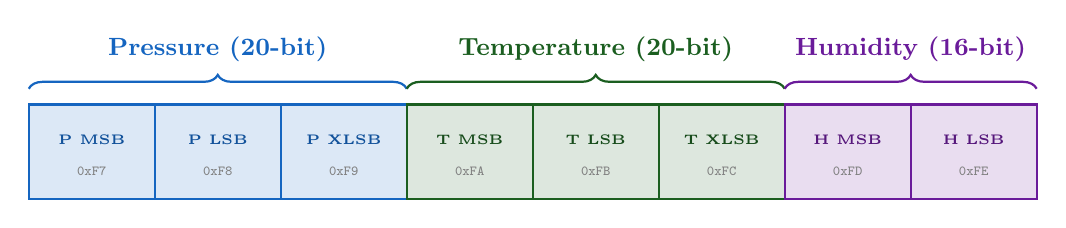
\begin{tikzpicture}
    \def\w{1.6}
    \foreach \i/\reg/\col/\lbl in {0/0xF7/accentblue/P MSB, 1/0xF8/accentblue/P LSB, 2/0xF9/accentblue/P XLSB, 3/0xFA/successgreen/T MSB, 4/0xFB/successgreen/T LSB, 5/0xFC/successgreen/T XLSB, 6/0xFD/hintpurple/H MSB, 7/0xFE/hintpurple/H LSB} {
        \draw[thick, fill=\col!15, draw=\col] (\i*\w, 0) rectangle +(\w, 1.2);
        \node[font=\tiny\bfseries, text=\col!80!black] at (\i*\w + \w/2, 0.75) {\lbl};
        \node[font=\tiny\ttfamily, text=gray] at (\i*\w + \w/2, 0.35) {\reg};
    }
    % Group braces
    \draw[decorate, decoration={brace, amplitude=5pt}, thick, accentblue] (0, 1.4) -- (3*\w, 1.4) node[midway, above=6pt, font=\small\bfseries, text=accentblue] {Pressure (20-bit)};
    \draw[decorate, decoration={brace, amplitude=5pt}, thick, successgreen] (3*\w, 1.4) -- (6*\w, 1.4) node[midway, above=6pt, font=\small\bfseries, text=successgreen] {Temperature (20-bit)};
    \draw[decorate, decoration={brace, amplitude=5pt}, thick, hintpurple] (6*\w, 1.4) -- (8*\w, 1.4) node[midway, above=6pt, font=\small\bfseries, text=hintpurple] {Humidity (16-bit)};
\end{tikzpicture}
\end{center}

\begin{codebox}[\faIcon{code}\ \ BME\_P280\_TEMP\_PRESS\_HUM() --- Read \& Display]
\begin{lstlisting}[style=CStyle]
void BME_P280_TEMP_PRESS_HUM(void)
{
    char MESSAGE[120];
    uint8_t VALUE[8];

    // Burst-read all 8 data registers at once
    I2C_READ_BYTES(BME_P280_REGISTER_PRESSURE_MSB, VALUE, 8);

    // Reconstruct 20-bit raw pressure (MSB[19:12], LSB[11:4], XLSB[3:0])
    int32_t P = ((int32_t)VALUE[0] << 12) |
                ((int32_t)VALUE[1] << 4)  |
                ((int32_t)VALUE[2] >> 4);

    // Reconstruct 20-bit raw temperature (same bit layout)
    int32_t T = ((int32_t)VALUE[3] << 12) |
                ((int32_t)VALUE[4] << 4)  |
                ((int32_t)VALUE[5] >> 4);

    // Reconstruct 16-bit raw humidity
    int32_t H = ((int32_t)VALUE[6] << 8) | VALUE[7];

    // Apply Bosch compensation formulas
    int32_t  TEMP     = BME_P280_BOSCH_TEMP_COMPENSATE(T);  // Must be first!
    uint32_t PRESSURE = BME_P280_BOSCH_PRESS_COMPENSATE(P);
    uint32_t HUMIDITY = BME_P280_BOSCH_HUM_COMPENSATE(H);

    // Format for display: separate integer and fraction parts
    int32_t  TEMP_FINAL = TEMP / 100;          // e.g., 25
    int32_t  TEMP_FRAC  = (TEMP < 0 ? -TEMP : TEMP) % 100; // e.g., 34
    uint32_t PRESS_HPA  = PRESSURE / 100;      // e.g., 1013
    uint32_t PRESS_FRAC = PRESSURE % 100;      // e.g., 25

    sprintf(MESSAGE, "| %6ld.%02ld C | %6lu.%02lu hPa | ...\r\n", ...);
    USART2_SendString(MESSAGE);
}
\end{lstlisting}
\end{codebox}

\begin{conceptbox}[20-bit Raw Data Reconstruction]
The BMP280 stores raw values across 3 bytes but only uses 20 bits:

\begin{center}
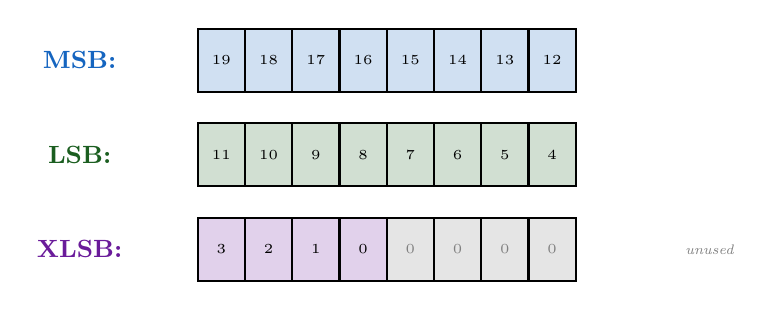
\begin{tikzpicture}
    \def\w{0.6}
    % MSB
    \node[font=\small\bfseries, text=accentblue] at (-1.5, 0.4) {MSB:};
    \foreach \i/\b in {0/19,1/18,2/17,3/16,4/15,5/14,6/13,7/12} {
        \draw[thick, fill=accentblue!20] (\i*\w, 0) rectangle +(\w, 0.8);
        \node[font=\tiny] at (\i*\w + \w/2, 0.4) {\b};
    }
    % LSB
    \node[font=\small\bfseries, text=successgreen] at (-1.5, -0.8) {LSB:};
    \foreach \i/\b in {0/11,1/10,2/9,3/8,4/7,5/6,6/5,7/4} {
        \draw[thick, fill=successgreen!20] (\i*\w, -1.2) rectangle +(\w, 0.8);
        \node[font=\tiny] at (\i*\w + \w/2, -0.8) {\b};
    }
    % XLSB
    \node[font=\small\bfseries, text=hintpurple] at (-1.5, -2) {XLSB:};
    \foreach \i/\b in {0/3,1/2,2/1,3/0} {
        \draw[thick, fill=hintpurple!20] (\i*\w, -2.4) rectangle +(\w, 0.8);
        \node[font=\tiny] at (\i*\w + \w/2, -2) {\b};
    }
    \foreach \i in {4,...,7} {
        \draw[thick, fill=gray!20] (\i*\w, -2.4) rectangle +(\w, 0.8);
        \node[font=\tiny, text=gray] at (\i*\w + \w/2, -2) {0};
    }
    \node[font=\tiny\itshape, text=gray] at (6.5, -2) {unused};
\end{tikzpicture}
\end{center}

Formula: \texttt{raw = (MSB << 12) | (LSB << 4) | (XLSB >> 4)}
\end{conceptbox}

% ╔══════════════════════════════════════════════════════════════════════════╗
% ║                SECTION 17: SENSOR CHECK                                 ║
% ╚══════════════════════════════════════════════════════════════════════════╝
\section{Function: \texttt{SENSOR\_CHECK()} --- Identification Routine}

\begin{codebox}[\faIcon{code}\ \ SENSOR\_CHECK() --- Verify and Identify the Sensor]
\begin{lstlisting}[style=CStyle]
void SENSOR_CHECK(void)
{
    // Step 1: Check if any device responds at address 0x76
    if (!I2C_DEVICE_ALIVE()) {
        USART2_SendString("[!] ACK not received. Going idle...\r\n");
        while (1); // Halt forever -- no point continuing
    }

    // Step 2: Read the chip ID register (0xD0)
    uint8_t id = I2C_READ_BYTE(BME_P280_REGISTER_CHIP_ID);

    // Step 3: Identify which sensor it is
    if (id == CHIP_ADDRESS_BME280)       // 0x60
        USART2_SendString("[*] BME280 detected (has humidity)\r\n");
    else if (id == CHIP_ADDRESS_BMP280)  // 0x58
        USART2_SendString("[*] BMP280 detected\r\n");
    else {
        // Unknown chip -- halt
        while (1);
    }
}
\end{lstlisting}
\end{codebox}

\begin{conceptbox}[BME280 vs BMP280 --- Key Differences]
\begin{center}
\renewcommand{\arraystretch}{1.3}
\begin{tabularx}{\textwidth}{>{\centering\bfseries\color{accentblue}\arraybackslash}p{3cm} >{\centering\arraybackslash}X >{\centering\arraybackslash}X}
\toprule
\rowcolor{accentblue!15}
\textbf{Feature} & \textbf{BMP280} & \textbf{BME280} \\
\midrule
Chip ID & \texttt{0x58} & \texttt{0x60} \\
\rowcolor{gray!5}
Temperature & \textcolor{successgreen}{\ding{51}} Yes & \textcolor{successgreen}{\ding{51}} Yes \\
Pressure & \textcolor{successgreen}{\ding{51}} Yes & \textcolor{successgreen}{\ding{51}} Yes \\
\rowcolor{gray!5}
Humidity & \textcolor{RedOrange}{\ding{55}} No & \textcolor{successgreen}{\ding{51}} Yes \\
Price & Lower & Slightly higher \\
\bottomrule
\end{tabularx}
\end{center}

\textbf{Note}: The problem statement mentions BME280, but the lab provides \textbf{BMP280}. The code handles both --- it checks the chip ID and adapts. For BMP280, humidity readings will show as 0 since the sensor lacks that capability.
\end{conceptbox}

% ╔══════════════════════════════════════════════════════════════════════════╗
% ║                SECTION 18: MAIN FUNCTION                                ║
% ╚══════════════════════════════════════════════════════════════════════════╝
\section{Function: \texttt{main()} --- Putting It All Together}

\begin{codebox}[\faIcon{code}\ \ The Main Function --- Execution Flow]
\begin{lstlisting}[style=CStyle]
int main(void)
{
    // Phase 1: Hardware Initialization
    PLL_CONFIG();     // Set system clock to 180MHz
    GPIO_CONFIG();    // Configure I2C + USART pins
    USART2_CONFIG();  // Set up serial debug output
    TIM6_CONFIG();    // Set up microsecond delay timer
    I2C_CONFIG();     // Initialize I2C1 peripheral at 100kHz

    USART2_SendString("LAB 02: BME/P-280 Communication by I2C\r\n");

    // Phase 2: Sensor Verification
    SENSOR_CHECK();   // Verify device is alive + identify chip

    // Phase 3: Load Calibration Data
    BME_P280_CALIBRATION_READ();  // Read factory calibration coefficients

    // Phase 4: Configure Sensor
    BME_P280_INIT();  // Reset, set oversampling, normal mode

    // Phase 5: Continuous Measurement Loop
    while (1) {
        BME_P280_TEMP_PRESS_HUM();  // Read + compensate + display
        delay_ms(1000);             // Wait 1 second
    }
}
\end{lstlisting}
\end{codebox}

\subsection{Complete Execution Flow Diagram}

\begin{center}
\begin{tikzpicture}[
    node distance=0.5cm,
    block/.style={rectangle, rounded corners=6pt, draw=#1, fill=#1!10, text width=10cm, minimum height=1cm, align=center, font=\small\bfseries, line width=1pt},
    arr/.style={-{Stealth[length=6pt]}, thick, color=#1},
]
    \node[block=accentblue] (p1) {\faIcon{wrench}\ \ PLL\_CONFIG $\rightarrow$ GPIO\_CONFIG $\rightarrow$ USART2\_CONFIG $\rightarrow$ TIM6\_CONFIG $\rightarrow$ I2C\_CONFIG};
    \node[font=\small\itshape\color{gray}, right=0.3cm of p1] {Hardware Init};
    
    \node[block=successgreen, below=of p1] (p2) {\faIcon{search}\ \ SENSOR\_CHECK: Send address $\rightarrow$ Check ACK $\rightarrow$ Read Chip ID};
    \node[font=\small\itshape\color{gray}, right=0.3cm of p2] {Verify Sensor};
    
    \node[block=hintpurple, below=of p2] (p3) {\faIcon{database}\ \ BME\_P280\_CALIBRATION\_READ: Load 24+7 bytes of factory calibration};
    \node[font=\small\itshape\color{gray}, right=0.3cm of p3] {Load Cal Data};
    
    \node[block=warnorange, below=of p3] (p4) {\faIcon{cog}\ \ BME\_P280\_INIT: Soft Reset $\rightarrow$ Config Filter $\rightarrow$ Set Oversampling $\rightarrow$ Normal Mode};
    \node[font=\small\itshape\color{gray}, right=0.3cm of p4] {Configure};
    
    \node[block=RedOrange, below=of p4] (p5) {\faIcon{sync-alt}\ \ LOOP: Read Raw Data $\rightarrow$ Compensate $\rightarrow$ Print via USART $\rightarrow$ Delay 1s $\rightarrow$ Repeat};
    \node[font=\small\itshape\color{gray}, right=0.3cm of p5] {Measure Loop};
    
    \draw[arr=accentblue] (p1) -- (p2);
    \draw[arr=successgreen] (p2) -- (p3);
    \draw[arr=hintpurple] (p3) -- (p4);
    \draw[arr=warnorange] (p4) -- (p5);
    
    % Loop arrow
    \draw[arr=RedOrange, rounded corners=10pt] (p5.east) -- ++(1,0) |- ([yshift=-0.3cm]p5.south) -- ++(0,-0.5) -- ++(-12,0) |- (p5.west);
\end{tikzpicture}
\end{center}

% ╔══════════════════════════════════════════════════════════════════════════╗
% ║                SECTION 19: I2C WAVEFORM SUMMARY                        ║
% ╚══════════════════════════════════════════════════════════════════════════╝
\section{I2C Communication Waveform Summary}

\begin{conceptbox}[Complete I2C Write Transaction: Writing 0x57 to Register 0xF4]
\begin{center}
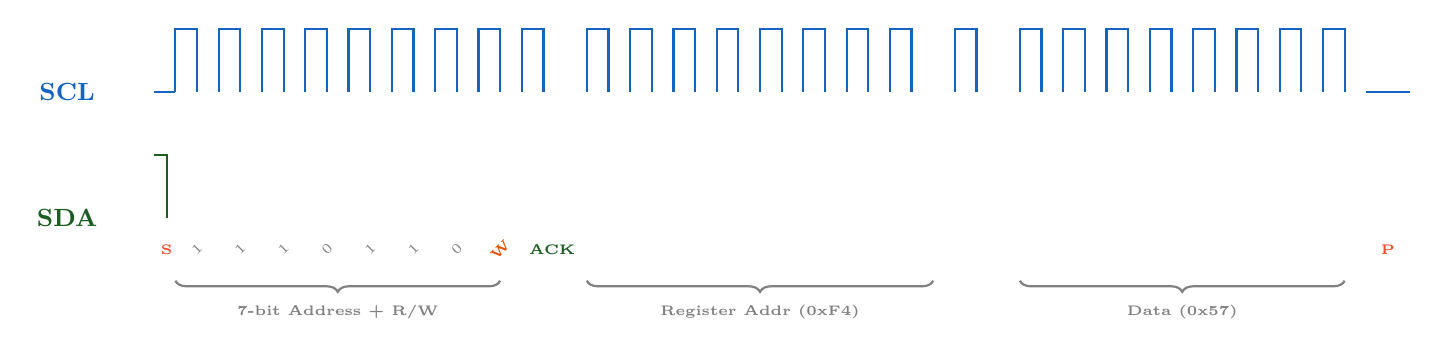
\begin{tikzpicture}[xscale=0.55, yscale=0.8]
    % SCL
    \node[font=\small\bfseries, text=accentblue] at (-2, 2) {SCL};
    \draw[thick, accentblue] (0,2) -- (0.5,2);
    % Clock pulses (simplified)
    \foreach \x in {0.5, 1.5, 2.5, 3.5, 4.5, 5.5, 6.5, 7.5, 8.5, 10, 11, 12, 13, 14, 15, 16, 17, 18.5, 20, 21, 22, 23, 24, 25, 26, 27} {
        \draw[thick, accentblue] (\x, 2) -- (\x, 3) -- (\x+0.5, 3) -- (\x+0.5, 2);
    }
    \draw[thick, accentblue] (28, 2) -- (29, 2);
    
    % SDA
    \node[font=\small\bfseries, text=successgreen] at (-2, 0) {SDA};
    
    % START
    \draw[thick, successgreen] (0, 1) -- (0.3, 1) -- (0.3, 0);
    \node[font=\tiny\bfseries, text=RedOrange] at (0.3, -0.5) {S};
    
    % Address bits (0x76 << 1 = 0xEC = 1110 1100)
    \node[font=\tiny, text=gray, rotate=45] at (1, -0.5) {1};
    \node[font=\tiny, text=gray, rotate=45] at (2, -0.5) {1};
    \node[font=\tiny, text=gray, rotate=45] at (3, -0.5) {1};
    \node[font=\tiny, text=gray, rotate=45] at (4, -0.5) {0};
    \node[font=\tiny, text=gray, rotate=45] at (5, -0.5) {1};
    \node[font=\tiny, text=gray, rotate=45] at (6, -0.5) {1};
    \node[font=\tiny, text=gray, rotate=45] at (7, -0.5) {0};
    \node[font=\tiny\bfseries, text=warnorange, rotate=45] at (8, -0.5) {W};
    \node[font=\tiny\bfseries, text=successgreen] at (9.2, -0.5) {ACK};
    
    % Labels
    \draw[decorate, decoration={brace, amplitude=4pt, mirror}, thick, gray] (0.5, -1) -- (8, -1) node[midway, below=5pt, font=\tiny\bfseries] {7-bit Address + R/W};
    \draw[decorate, decoration={brace, amplitude=4pt, mirror}, thick, gray] (10, -1) -- (18, -1) node[midway, below=5pt, font=\tiny\bfseries] {Register Addr (0xF4)};
    \draw[decorate, decoration={brace, amplitude=4pt, mirror}, thick, gray] (20, -1) -- (27.5, -1) node[midway, below=5pt, font=\tiny\bfseries] {Data (0x57)};
    
    % STOP
    \node[font=\tiny\bfseries, text=RedOrange] at (28.5, -0.5) {P};
\end{tikzpicture}
\end{center}

\textbf{S} = START condition, \textbf{P} = STOP condition, \textbf{W} = Write bit (0), \textbf{ACK} = Acknowledge from slave.
\end{conceptbox}

% ╔══════════════════════════════════════════════════════════════════════════╗
% ║                SECTION 20: QUICK REFERENCE                              ║
% ╚══════════════════════════════════════════════════════════════════════════╝
\section{Quick Reference --- Function Summary Table}

\begin{center}
\renewcommand{\arraystretch}{1.4}
\small
\begin{tabularx}{\textwidth}{>{\ttfamily\bfseries\color{deepblue}\arraybackslash}p{4.2cm} >{\centering\arraybackslash}p{2.5cm} X}
\toprule
\rowcolor{accentblue!20}
\textbf{Function} & \textbf{Category} & \textbf{Purpose} \\
\midrule
PLL\_CONFIG() & Clock & Sets system clock to 180\,MHz via PLL using HSE \\
\rowcolor{gray!5}
GPIO\_CONFIG() & GPIO & Configures PA2 (USART TX), PB8 (SCL), PB9 (SDA) \\
USART2\_CONFIG() & Debug & Initializes USART2 at 115200 baud for serial output \\
\rowcolor{gray!5}
USART2\_SendString() & Debug & Sends a null-terminated string character by character \\
TIM6\_CONFIG() & Timer & Configures TIM6 for 1\,$\mu$s resolution free-running \\
\rowcolor{gray!5}
delay\_us() / delay\_ms() & Timer & Blocking microsecond / millisecond delay \\
I2C\_CONFIG() & I2C & Initializes I2C1 at 100\,kHz standard mode \\
\rowcolor{gray!5}
I2C\_WRITE\_BYTE() & I2C & Writes one byte to a specified register \\
I2C\_READ\_BYTE() & I2C & Reads one byte from a specified register \\
\rowcolor{gray!5}
I2C\_READ\_BYTES() & I2C & Burst-reads multiple bytes from consecutive registers \\
I2C\_DEVICE\_ALIVE() & I2C & Checks if slave responds with ACK \\
\rowcolor{gray!5}
SENSOR\_CHECK() & Sensor & Verifies and identifies BMP280 / BME280 \\
CALIBRATION\_READ() & Sensor & Loads factory calibration coefficients \\
\rowcolor{gray!5}
BME\_P280\_INIT() & Sensor & Resets sensor, configures oversampling and mode \\
TEMP\_COMPENSATE() & Math & Converts raw ADC to temperature ($^\circ$C $\times$ 100) \\
\rowcolor{gray!5}
PRESS\_COMPENSATE() & Math & Converts raw ADC to pressure (Pa) \\
HUM\_COMPENSATE() & Math & Converts raw ADC to humidity (\%RH $\times$ 1024) \\
\rowcolor{gray!5}
TEMP\_PRESS\_HUM() & Main & Reads, compensates, and prints all sensor data \\
\bottomrule
\end{tabularx}
\end{center}

% ╔══════════════════════════════════════════════════════════════════════════╗
% ║                SECTION 21: COMMON EXAM QUESTIONS                        ║
% ╚══════════════════════════════════════════════════════════════════════════╝
\section{Common Lab Exam Questions \& Answers}

\begin{tcolorbox}[enhanced, colback=accentblue!5, colframe=accentblue, arc=6pt, title={\large\faIcon{question-circle}\ \ Frequently Asked Questions}, coltitle=white, colbacktitle=accentblue, fonttitle=\bfseries, breakable]

\textbf{\textcolor{accentblue}{Q1: Why do I2C lines use open-drain with pull-ups?}}\\
Because I2C is a \textit{wired-AND} bus. Multiple devices share the same wires. Open-drain prevents short circuits when two devices try to control the line simultaneously. Pull-ups keep the default state HIGH.

\vspace{0.4cm}
\textbf{\textcolor{accentblue}{Q2: What is the difference between START and Repeated START?}}\\
A \textbf{START} begins a new transaction after the bus is idle. A \textbf{Repeated START} changes direction (write$\rightarrow$read) \textit{without releasing the bus}. This prevents another master from hijacking the bus between your write (register address) and read (data) phases.

\vspace{0.4cm}
\textbf{\textcolor{accentblue}{Q3: Why must temperature be compensated before pressure?}}\\
Because the pressure formula depends on \texttt{t\_fine}, a global variable set during temperature compensation. Pressure measurements are temperature-dependent --- warm air exerts different pressure than cold air at the same altitude.

\vspace{0.4cm}
\textbf{\textcolor{accentblue}{Q4: How is the I2C address determined to be 0x76?}}\\
The BMP280 has a configurable address pin (SDO). When SDO is connected to \textbf{GND}, the address is \texttt{0x76}. When connected to \textbf{VCC}, it becomes \texttt{0x77}. This allows two BMP280 sensors on the same I2C bus.

\vspace{0.4cm}
\textbf{\textcolor{accentblue}{Q5: What does the IIR filter do in the BMP280?}}\\
The IIR (Infinite Impulse Response) filter smooths pressure readings by weighing previous measurements. Higher coefficients (like x16 in our code) produce smoother data but slower response. This is ideal for weather stations but not for fast-changing altitude measurements.

\vspace{0.4cm}
\textbf{\textcolor{accentblue}{Q6: Why do we read SR2 after checking ADDR flag?}}\\
It's an STM32 hardware design requirement. The ADDR flag is cleared by the specific sequence of reading SR1 then SR2. Forgetting to read SR2 leaves ADDR set, and the I2C peripheral will hang waiting for the flag to be cleared.

\vspace{0.4cm}
\textbf{\textcolor{accentblue}{Q7: What's the difference between BMP280 and BME280?}}\\
BMP280 measures \textbf{temperature and pressure} only. BME280 adds \textbf{humidity sensing}. They are pin-compatible and use the same I2C protocol, but have different chip IDs (0x58 vs 0x60).

\vspace{0.4cm}
\textbf{\textcolor{accentblue}{Q8: Why is CCR set to 225?}}\\
CCR (Clock Control Register) determines SCL frequency. For 100\,kHz standard mode with 45\,MHz APB1 clock: CCR = 45,000,000 / (2 $\times$ 100,000) = 225. Each half-period of SCL = 225 $\times$ (1/45MHz) = 5\,$\mu$s, so full period = 10\,$\mu$s = 100\,kHz.
\end{tcolorbox}

\vspace{1cm}
\begin{center}
\textcolor{accentblue}{\rule{0.8\linewidth}{1.5pt}}\\[0.5cm]
{\Large\bfseries\textcolor{deepblue}{Good Luck on Your Lab Exam! \faIcon{star}}}\\[0.3cm]
{\small\textcolor{gray}{This document covers every function in the bare-metal I2C BMP280 implementation.}}\\
{\small\textcolor{gray}{Generated for CSE-2206 Microcontroller Lab --- Assignment 03, LAB\_02(A).}}
\end{center}

\end{document}
